\documentclass[a4paper, 12pt]{article}
\usepackage{siunitx}
\usepackage[style=listdotted,toc,nopostdot,acronym,nomain]{glossaries}
\usepackage{amsmath}
\usepackage{amsfonts}
\usepackage{listliketab}
\usepackage{listings}
\usepackage{booktabs}
\usepackage{url}
\usepackage{cite}
\usepackage{tikz}
\usetikzlibrary{decorations.markings}
\usetikzlibrary{arrows,positioning, automata, shadows, fit, shapes}
\usepackage{color}
\usepackage{bm}
\usepackage{ragged2e}
\usepackage{pgfplots}
\pgfplotsset{compat=1.5}
\usepackage{float}
\usepackage{courier}
\usepackage{setspace}
\usepackage{multicol}
\usepackage[margin=2.7cm]{geometry}
\usepackage{mathtools}
\usetikzlibrary{external}
\tikzexternalize
\DeclarePairedDelimiter\abs{\lvert}{\rvert}%
\makeatletter
\let\oldabs\abs
\def\abs{\@ifstar{\oldabs}{\oldabs*}}
\makeatother
\makeglossaries
\newacronym{spa}{SPA}{stationary phase approximation}
\newacronym{iec}{IEC}{interlayer exchange coupling}
\newacronym{gmr}{GMR}{giant magneto-resistance}
\newacronym{stt}{STT}{spin transfer torque}
\newacronym{mram}{MRAM}{magnetoresistive random access memory}
\newacronym{hdd}{HDD}{hard disk drive}
\newacronym{fm}{FM}{ferromagnetic}
\newacronym{af}{AF}{anti-ferromagnetic}
\newacronym{cip}{CIP}{current in-plane}
\newacronym{cpp}{CPP}{current perpendicular to plane}
\newacronym{tmr}{TMR}{tunneling magneto-resistance}
\newacronym{mtj}{MTJ}{magnetic tunnel junctions}
\newacronym{pm}{PM}{polarising magnet}
\newacronym{fcc}{fcc}{face-centre cubic}
\newacronym{bcc}{bcc}{body-centre cubic}
\newacronym{nnn}{nnn}{next-nearest neighbour}
\newacronym{nn}{nn}{nearest neighbour}
\newacronym{sc}{SC}{simple cubic}
\newacronym{sgf}{SGF}{surface Green's function}
\newacronym{ldos}{LDOS}{local density of states}
\newacronym{sm}{SM}{switching magnet}
\newacronym{fft}{FFT}{fast fourier transform}
\newacronym{mtgf}{MTGF}{M\"{o}bius transformed Green's function}
\newacronym{2dbz}{2DBZ}{two dimensional Brillouin zone}
\newcommand{\site}[1]{\textsuperscript{\textcolor{blue}{\cite{#1}}}}
% to do: replace all references to CP routine to that of Authors own.
\author{Alexander Durie}
\begin{document}
	\begin{titlepage}
		\begin{figure}[H]
			\centering
			
\includegraphics[width=2in]{OU_logo.jpg}
		\end{figure}
		\begin{center}
			\vspace{2cm}
			\huge{The Open University}\\[1.5cm]
			\Large
			First Year Report\\[4mm]
			\linethickness{1pt}\line(1,0){440}
			\\
			\LARGE\bf The Origin and Significance of the Phase\\ of out of plane Exchange Coupling
			\\[-4mm]

			\line(1,0){440}
		\end{center}
		\begin{multicols}{2}
			\justify \underline{Author:}\\[1mm]
			\footnotesize Alexander DURIE\\[17mm]
			\begin{flushright}
				\normalsize\underline{Supervisor:}\\[1mm]
				\footnotesize{Dr. Andrey UMERSKI}\\[3mm]
				\normalsize\underline{Secondary Supervisor:}\\[1mm]
				\footnotesize Prof. Uwe GRIMM\\[3mm]
				\normalsize\underline{Third Party Monitor:}\\[1mm]
				\footnotesize Dr. Toby O'NEILL
			\end{flushright}
		\end{multicols}
		\vspace{5cm}
		\large\centering\today
	\end{titlepage}
	\newpage
	\tableofcontents

	\newpage
	\printglossaries
	\newpage
	\section{Author's developments since registration}
	The following programming languages have been studied, listed in order of fluency. Libraries studied are given in subentries. The references given here indicate the documentation studied.
	\begin{multicols}{2}
	\begin{itemize}
		\item C++98\textsuperscript{\textcolor{blue}{\cite{acc, alex}}}, C++11\site{c++ref}, C++14
			\begin{itemize}
				\item Eigen\site{eigen}
				\item GNU Scientific Library\site{gsl}
				\item OpenMP\site{openmp}
				\item Blaze\site{blaze}
				\item Boost
				\item SymbolicC++\site{symbolicc}
				\item CBLAS
				\item CLAPACK
			\end{itemize}
		\item Julia\site{julia}
			\begin{itemize}
				\item SymPy
			\end{itemize}
		\item Python2.7\site{python}, Python3.4
			\begin{itemize}
				\item SymPy\site{sympy}
				\item SciPy\site{scipy}
				\item NumPy\site{numpy}
			\end{itemize}
			\columnbreak
		\item Fortran95
		\item C
			\begin{itemize}
				\item GNU Scientific Library
				\item CBLAS
				\item CLAPACK
			\end{itemize}
		\item Maple 2015 programming blocks
		\item Scilab\site{scilab}
		\item Octave\site{octave}
		\item Haskell\site{haskell}
		\item Perl
		\item Go
	\end{itemize}
\end{multicols}
The following software packages have been studied with a brief description of their purposes
	\begin{itemize}
		\item Maple 2015 \quad - \quad {\it computer algebra package}
		\item VIM\site{vim} \quad - \quad {\it text editor with powerful keybindings}
			\begin{itemize}
				\item Latex-Suite \quad - \quad {\it \LaTeX package with additional keybindings specific to \LaTeX}
			\end{itemize}
		\item TeXMaker \quad - \quad {\it a \LaTeX editor}
		\item QTIplots \quad - \quad {\it provides graphical output from raw data}
		\item \LaTeX \quad - \quad {\it a powerful typesetting language}
			\setlength\itemsep{1em}
			\begin{itemize}
				\item Ti\textit{k}Z\site{tikz} \quad - \quad {\it provides graphics through a coding interface, all figures in this document are {\rm Ti\textit{k}Z \it images}}
				\item pgfplots\site{pgf} \quad - \quad {\it built from {\rm Ti\textit{k}Z}, a package that generates graphs within \LaTeX, all graphs in this document are built using pgfplots}
				\item Bib\TeX \quad - \quad {\it a bibliographical package}
				\item glossaries \quad - \quad {\it generates glossaries and lists of acronyms if required, by running a Perl script}
			\end{itemize}
	\end{itemize}
	Further skills developed include learning to touch-type
\\	Miscellaneous tools used include the LLVM Clang compiler for C++, the GNU Debugger, Google gperftools and valgrind.
The following programs have been written with a brief description of their purposes

\begin{itemize}
	\item{C++}
		\begin{itemize}
			\setlength\itemsep{1em}
			\item cunningham\_points\_integration.h \quad-\quad {\it header file that performs \gls{2dbz} integration, more details are given in the Appendix}
			\item interp.cpp \quad-\quad {\it takes raw data as input and interpolates results}
			\item analytic\_conductance\_trilayer\_landauer.cpp \quad-\quad {\it calculates the conductance using the Landauer formalism using analytical methods}
			\item numerical\_conductance\_trilayer\_landauer.cpp \quad-\quad {\it calculates the conductance using the Landauer formalism using direct calculations}
			\item LDOS\_SGF.cpp \quad-\quad {\it calculates the \gls{ldos} of a semi-infinite crystal at user specified atomic planes from the surface, using Equation \eqref{rho}}
			\item trilayer\_conductance\_kubo.cpp \quad-\quad {\it calculates the charge current using the Kubo formula\site{kubo1} in the spinless one-band \gls{sc} model}
			\item spincurrent\_4-layer\_$<$j\_n-1$>$2\_keldysh.cpp \quad-\quad {\it calculates the equilibrium term at zero bias of the spincurrent (Equation \eqref{keldysh}) under the Keldysh Formalism\site{keldysh_1} in one-band \gls{sc}, the integration over energy has been bypassed by expanding Equation \eqref{fermi} as a Taylor series to first order. At zero bias, the integration of the remaining term at zero-bias is a delta-function.}
			\item spinenergy.cpp \quad-\quad {\it calculates the transport term, Equation \eqref{keldysh_1} of the spincurrent under the Keldysh formalism in the one-band \gls{sc} system. Difficulties with convergence of the energy integral, as yet unresolved}
			\item EC\_integration\_GSL.cpp \quad-\quad {\it  calculates the \gls{iec} in one-band \gls{sc} by calculating Equation \eqref{exchange} directly. Convergence problems not yet resolved}
			\item matsubara\_method\_EC\_trilayer.cpp \quad-\quad {\it calculates the \gls{iec} in one-band \gls{sc} using Equation \eqref{matsu}}
			\item EC\_SPA\_final\_efficient.cpp \quad-\quad {\it calculates the \gls{iec} in one-band \gls{sc} using the \gls{spa} (Equation \eqref{SPA_2}) where the Fourier components are obtained directly. Utilises OpenMP for concurrency}
			\item EC\_SPA\_FFT.cpp \quad-\quad {\it calculates the \gls{iec} in one-band \gls{sc} using the \gls{spa} (Equation \eqref{SPA_2}) where the Fourier coefficients are obtained through an inverse \gls{fft}. Utilises OpenMP for concurrency}
			\item EC\_SPA\_mobius.cpp \quad-\quad {\it calculates the \gls{iec} in one-band \gls{sc} using the \gls{spa} (Equation \eqref{SPA_2}) where the Fourier coefficients are obtained from Equation \eqref{fs}. Utilises OpenMP for concurrency}
			\item EC\_2-band.cpp \quad-\quad {\it calculates the \gls{iec} in a two-band trilayer using Equation \eqref{matsu}}
		\end{itemize}
	\item{Fortran}
		\begin{itemize}
			\setlength\itemsep{1em}
			\item conductor\_approx\_with\_r.f90 \quad-\quad {\it calculates the charge current for a trilayer with a conducting spacer using the Landuaer formalism}
			\item insulator\_approx\_with\_$\rm r^\wedge$2.f90 \quad-\quad {\it calculates the charge current for a trilayer with an insulator spacer using the Landuaer formalism}
			\item analytic\_trilayer\_with\_conductor.f90 \quad-\quad {\it calculates the charge current for a trilayer with a conducting spacer using analytic derivations using the Landauer formalism}
		\end{itemize}
\end{itemize}
In addition to the equations derived in this document, the following known results have also been derived by the Author;
\begin{itemize}
	\item{Equilibrium Keldysh term without the energy integral derived from Equation \eqref{keldysh}}
	\item{Partial conductance of a trilayer with an insulating spacer, Equation (3) of \textcolor{blue}{\cite{Mathon2016}}}
	\item{Analytic form of Total conductance in a trilayer with an insulating spacer using the Landauer formalism, Equation (6) of \textcolor{blue}{\cite{Mathon2016}}}
	\item{Analytic form of Total Conductance in a trilayer with a conducting spacer using the Landauer formalism by considering $\Gamma$-point and cutoff-point terms using higher order stationary phase approximations and cutoff point approximations and further Fourier terms. These were written up in an unpublished document\site{me}}
	\item{Partial conductance of a 4-layer system in the Landuaer formalism in a conductor}
	\item{Creation of a Maple document that calculates the partial conductance in the Landauer formalism in a conductor for an arbitrary number of layers using a programming block}
	\item{Further tight binding}
		\begin{itemize}
			\item{calculation of Fermi surfaces of \gls{sc}, \gls{fcc} and \gls{bcc}}
			\item{\gls{sc} 2-band model}
			\item{\gls{fcc} in a two atom basis in a pseudo one-dimensional lattice}
		\end{itemize}
\end{itemize}
A great deal of the programs written and formulae derived were done so in conjunction with Maple worksheets.
	\newpage
	\begin{abstract}
		The system explored is a pseudo one-dimensional \gls{cpp} magnetic multilayer. The Green's function formalism is used here, as this offers a means of providing complete and accurate results comparable if correctly modeled to experiment. This review begins with a brief history of the subject area, moving on to a description of the necessary tools needed, such as the method of Tight Binding and derivations of closed form Green's functions. These methods are then applied to the \gls{iec} firstly in its full form simplified by the method of Matsubara, followed by the derivation of an analytical method. The origin of the phase of \gls{iec} is then discussed and derived to be followed by a conclusion and a plan for future work. The paper concludes with numerical integration routines described in the Appendix.
	\end{abstract}
	\section{Introduction}
	\subsection{History}
	There has been significant interest in the field of spintronics for the past three decades. This interest began with the discovery that the resistance of a multilayer comprising of alternating sets of thin magnetic and equally thin non-magnetic metallic layers was much lower when the magnetic moments of the layers were parallel compared to the anti-parallel case\textcolor{blue}{\textsuperscript{\cite{rev3, GMR1, GMR2}}}. This is explained by the fact that if a device is constructed on the nanoscopic scale, such that the thickness is smaller than the spin diffusion length, spin can flow through this device with some memory of it's orientation. A magnet by definition polarises spin, so that spincurrent can be modelled as if flowing through two independent wires. The up an down spin carriers are scattered at different rates at layer interfaces and the total resistance of the structure depends on the magnetic configuration of all magnetic components, which in turn can be modified by an applied magnetic field thus the resistance can be manipulated by this field. 
This is \gls{gmr}. The so-called {\it optimistic magneto-resistance ratio} is defined by
	\begin{equation}
		\frac{\Delta R}{R}=\frac{R^{\uparrow \downarrow}-R^{\uparrow\uparrow}}{R^{\uparrow\uparrow}}
	\end{equation}
	Where $R^{\uparrow\uparrow}$, $R^{\uparrow\downarrow}$ are the resistances of the saturated \gls{fm} configuration and \gls{af} configuration respectively. 
	A second significant finding in the field was the discovery by Parkin \textit{et. al.}\textcolor{blue}{\textsuperscript{\cite{Parkin}}} of \gls{iec} 
	which describes the fact that the relative orientation of magnetic moments of coupled magnetic layers separated by a nonmagnetic spacer, is dependent on the spacer layer thickness and in fact oscillates between \gls{fm} and \gls{af} regimes as a function of spacer layer thickness. 
	The early \gls{gmr} devices were built with \gls{cip} and were developed very quickly into commercial devices, with IBM in 1997 producing \gls{hdd} read heads that utilised this effect to allow a new upper bound on the number of bits read/writable per unit area. In fact the storage density increased from $0.1$ to $100$Gbit/i$\rm n^2$ between 1991 and 2003\textcolor{blue}{\textsuperscript{\cite{Mathon2016}}}.  
	\par In 2001, two groups simultaneously described the theory of a new system\textsuperscript{\textcolor{blue}{\cite{tunnel1,tunnel2}}} which is designed with \gls{cpp} . Their original system was a trilayer with ferromagnetic leads made from Fe, and an insulating spacer material made from crystalline MgO. From a theoretical standpoint, these materials are excellent to study since their Brillouin zones are of very similar sizes meaning growth from one material to another is easy to model since only a change in potentials is required. The magneto-resistance produced by this scheme is known as \gls{tmr} since the electrons must tunnel through the MgO potential barrier making this an entirely quantum mechanical effect. \gls{gmr} predicts an optimistic magneto-resistance ratio as high as $50\%$ whereas \gls{tmr} predicts a ratio as high as $1000\%$.
	The success of the \gls{tmr} system, which was confirmed experimentally in 2004\textsuperscript{\textcolor{blue}{\cite{2004,2004P}}}, led to a very rapid appearance of these \gls{tmr} read heads in commercial \gls{hdd}'s making their debut appearance in 2007. As a result, these read heads are now constructed in every modern \gls{hdd}. The 2004 experiments were unable to replicate the same MR ratio reaching only as high as $200\%$ at room temperature. This is due to the difficulty in engineering 'clean' epitaxial surfaces free from defect, which the original \gls{mtj} were sensitive to. In 2008 experimentalists were able to get \gls{tmr} ratios as high as $1144\%$ at 5K\textsuperscript{\textcolor{blue}{\cite{1100}}}.
	\par It	has been well known for some time that altering the magnetic configuration of a magnetic multilayer influences the charge current flowing through it. More recently it has been recognised that conversely, by passing a strong charge current through a magnetic trilayer, the current becomes spin-polarised when passing through the pinned magnet so that a spin current flows through the spacer to the opposing ferromagnet (the switching magnet). The spin current is absorbed by the \gls{sm} exerting a force known as \gls{stt}. If the \gls{stt} is high enough, the \gls{sm} undergoes a total reversal of magnetisation in an effect known as current-induced switching of magnetisation, which remains a very active field due to its obvious commercial potential in \gls{mram}\textsuperscript{\textcolor{blue}{\cite{stt}}}, a non-volatile form of random access memory with potential to become a universal memory\site{universal}, a form of data storage replacing the separate CPU cache, RAM and \gls{hdd} storage. \gls{mram} is non-volatile since the \gls{sm}'s retain their configuration in the absence of charge current. It remains a problem that too much heat is generated in these devices and this is of current research interest.
	\par In the absence of charge current in a magnetic multilayer, there remains a net flow of spin current between the two magnetic layers, provided the magnets are out of alignment. This is \gls{iec}. Given the phenomenon exists without the expense of a charge current, \gls{iec} has been under active research due to possible implications such as \gls{mram} or CPU chips without the same heat generation due to lack of flowing charge. Recently \gls{iec} has fallen out of favour, with later research has focussing on \gls{stt} and current induced switching of magnetisation. In 1998, Ebels \textit{et. al.} found by experiment induced phase shifts in \gls{iec} in magnetic trilayers, by doping the magnetic layers\site{ebels}. Due to the limited interest at the time, it is likely the potential implications such as switching induced by altering the phase of \gls{iec} were not recognised at the time. Recently, one of the pioneers of \gls{cpp} \gls{tmr} devices made this observation and revives the mechanism for doing so\textsuperscript{\textcolor{blue}{\cite{AUphase}}}. This is the main research focus here.
	\section{Green's Function Formalism}
	\subsection{Method of Tight Binding}\label{tb}
	The Method of Tight Binding is a convenient framework to use in this context as it models very well the potentials arising in atoms in a regular periodic structure. 
	In an infinite periodic structure a translation from one crystal site to another leaves the structure as a whole unchanged since each site is identical. A structure of this nature is referred to as Bloch-like\textsuperscript{\textcolor{blue}{\cite{kittel_1996}}}.
	The position vector of each atomic site is given by $\bf R$,
		where ${\bf R} = \sum_j^\chi n_j{\bf a}_i$ can describe the position of any lattice site with integers $n_j$, primitive translation vectors ${\bf a}_j$ and $\chi$ is equal to the dimension of $\bf R$ \\ 
		\\In the tight binding formalism, the energy eigenvalues are given by 
		\begin{equation}
			\varepsilon({\bf k}) = \frac{\langle {\bf k}|{\bf H}|{\bf k} \rangle}{\langle\bf k|k\rangle}
		\end{equation}
		In order to diagonalise the matrix Hamiltonian, $\bf H$, the transformation from real space to Hilbert space is required
		\begin{equation}\label{kkk}
			|{\bf k}\rangle = \frac{1}{\sqrt{N}}\sum_{\bf R = -\infty}^\infty e^{i{\bf k}\cdot \bf R} |\bf R\rangle
		\end{equation}
		where the summation is over every lattice point. The position of any site in the reciprocal lattice is given by ${\bf k} = \sum_i^\chi k_i{\bf b}_i$ with integers $k_i$ and primitive translation vectors ${\bf b}_i$ determined such that 
		\begin{equation}
		{\bf b}_i\cdot {\bf a}_j = 2\pi \delta_{i j}
			\label{ab}
		\end{equation}
Where since 
		\begin{equation}
			\langle{\bf R}|{\bf \acute{R}}\rangle = \delta_{\bf R \acute{R}}
		\end{equation}
		It follows that
		\begin{equation}
			\label{kk}
			\langle{\bf k}|{\bf \acute{k}}\rangle = \frac{1}{N}\sum_{\bf R \acute{R}} e^{-i{\bf k}\cdot{\bf R}}e^{i{\bf \acute{k}}\cdot{\bf \acute{R}}} \langle{\bf R | \acute{R}}\rangle \equiv \frac{1}{N}\sum_{\bf R} e^{-i{\bf R\cdot(k-\acute{k})}}=\delta_{\bf k \acute{k}}
		\end{equation}
		Assuming a small set of nearby atoms overlap with non-negligable results, all elements of the Hamiltonian are zero, except
		\begin{equation}\label{u}
			\langle{\bf R}|{\bf H}|{\bf R}\rangle = \bf u
		\end{equation}
		the onsite potential, and 
		\begin{equation}\label{t}
			\langle{\bf R}|{\bf H}|{\bf R}\pm {\bf d}\rangle = \bf t
		\end{equation}
		where $\bf d$ is the set of position vectors of the all the non-negligable neighbouring terms. $\bf t$ is the set of hopping matrices who's strength varies depending on the binding distance to the onsite term. Models involving multiple energy bands or multiple bases per site require that $\bf t, u$ are matrices. 
		\\[2mm]Thus
		\begin{equation}
			\langle{\bf R}|{\bf H}|{\bf \acute{k}}\rangle = \frac{1}{\sqrt{N}}\sum_{\bf \acute{R}}\langle{\bf {R}}|{\bf H}|{\bf \acute{R}}\rangle e^{i\bf \acute{k}\cdot \acute{R}}= \frac{1}{\sqrt{N}}e^{i\bf \acute{k}\cdot R}\left({\bf u}+\sum_{{\bf d }\in {\bf R}}e^{i{\bf k \cdot d}}\langle{\bf R}|{\bf H}|{\bf R}\pm {\bf d}\rangle\right)
		\end{equation}
		and
		\begin{equation}\label{sumtb}
			\langle{\bf k}|{\bf H}|{\bf \acute{k}}\rangle = \frac{1}{N}\sum_{\bf R} e^{i\bf R\cdot (\acute{k}-k)}\left( {\bf u} + \sum_{{\bf d}\in {\bf R}}e^{i{\bf k \cdot d}}\langle\bf 0|H|d\rangle\right) = \delta_{\bf k \acute{k}}\left( {\bf u} + \sum_{{\bf d}\in {\bf R}}e^{i{\bf k \cdot d}}\langle\bf 0|H|d\rangle\right)
		\end{equation}
		where Equation \eqref{kk} is used.
		The energy eigenvalues are thus
		\begin{equation}
			\varepsilon({\bf k})= {\bf u} + \sum_{{\bf d}\in {\bf R}}e^{i{\bf k \cdot d}}\langle\bf 0|H|d\rangle
			\label{tight}
		\end{equation}
	\subsubsection{One-band model 1D example}
	\begin{figure}[H]
	\begin{center}
		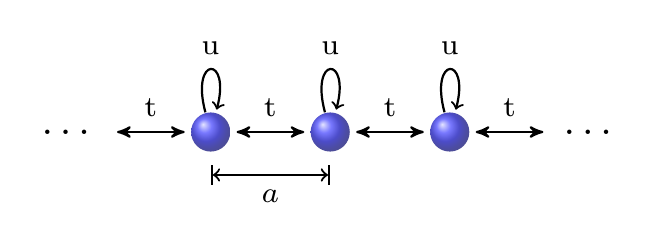
\begin{tikzpicture}[scale=1.5, every node/.style={scale=1.5}]
		\node[circle, opacity=0.7, shading=ball] (1){};
		\node[circle, opacity=0.7, shading=ball] (2)[left=of 1]{};
		\node[circle, opacity=0.7, shading=ball] (3)[right=of 1]{};
		\node (4)[right=of 3]{\dots};
		\node (5)[left =of 2]{\dots};
		\node (6)[below =of 1, yshift = 0.6cm]{};
		\node (7)[below =of 2, yshift = 0.6cm]{};
		\draw[<->,thick,>=stealth',shorten <=2pt,shorten >=2pt] (1.east)--(3.west) node[midway,above] {\scriptsize{t}};
		\draw[<->,thick,>=stealth',shorten <=2pt,shorten >=2pt] (3.east)--(4.west) node[midway,above] {\scriptsize t};
		\draw[<->,thick,>=stealth',shorten <=2pt,shorten >=2pt] (5.east)--(2.west) node[midway, above] {\scriptsize t};
		\draw[<->,thick,>=stealth',shorten <=2pt,shorten >=2pt] (2.east)--(1.west) node[midway, above] {\scriptsize t};
		\draw (1) edge [loop above, <->, thick] node {\scriptsize u} (1);
		\draw (2) edge [loop above, <->, thick] node {\scriptsize u} (1);
		\draw (3) edge [loop above, <->, thick] node {\scriptsize u} (1);
		\draw[|<->|, thick] (6.center)--(7.center) node[midway, below] {$\scriptstyle a$};
	\end{tikzpicture}
\end{center}
\caption{\footnotesize Depiction of an infinite chain of atoms in one dimension separated by $a$ showing the self energy u, and the hopping energy t.}\label{monochain}
\end{figure}
	In the one-band model in one dimension, all the vector values become scalar and the position of a given lattice site is $R=na$ and $d = \pm a$. As such, Eq. \eqref{tight} becomes
	\begin{equation}
		\varepsilon = {\rm u + t}(e^{i{\rm k}a} + e^{-i{\rm k}a}) = {\rm u}+2{\rm t}\cos{{\rm k}a}
	\end{equation}
	\subsubsection{One-band model \gls{bcc} example}\label{3dbcc}

	\begin{figure}[H]
	\begin{center}
		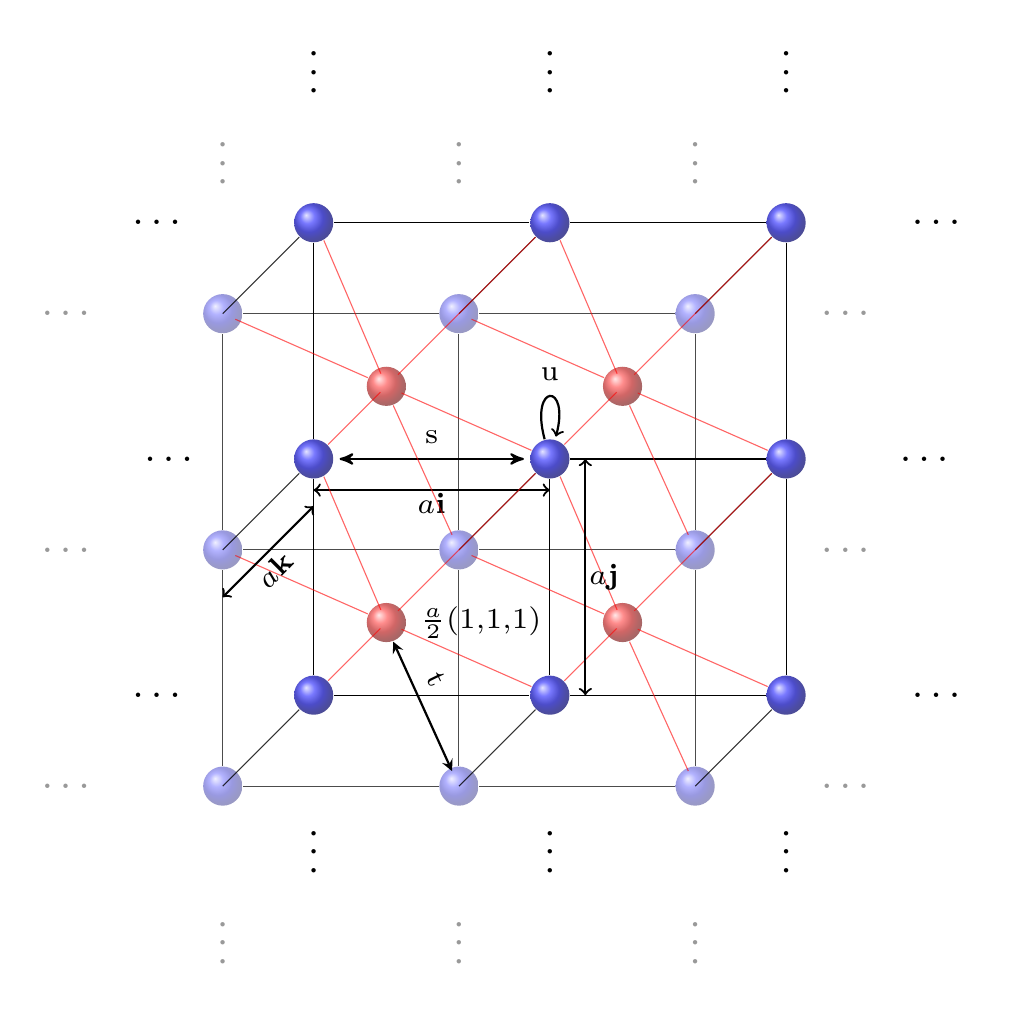
\begin{tikzpicture}[scale=1.5, every node/.style={scale=1.5}]
			\node[circle, opacity=0.7, shading=ball] (1) at (0,0,0) {};
		\node[circle, opacity=0.7, shading=ball] (2) at (-2,0,0){};
		\node[circle, opacity=0.7, shading=ball] (3) at (2,0,0){};
		\node (1.1)[circle, opacity = 0.4, shading = ball] at (0,0,2) {};
		\node[circle, opacity=0.4, shading=ball] (2.1) at (-2,0,2){};
		\node[circle, opacity=0.4, shading=ball] (3.1) at (2,0,2){};
			\node[circle, opacity=0.7, shading=ball] (1.2) at (0,2,0) {};
		\node[circle, opacity=0.7, shading=ball] (2.2) at (-2,2,0){};
		\node[circle, opacity=0.7, shading=ball] (3.2) at (2,2,0){};
		\node (1.12)[circle, opacity = 0.4, shading = ball] at (0,2,2) {};
		\node[circle, opacity=0.4, shading=ball] (2.12) at (-2,2,2){};
		\node[circle, opacity=0.4, shading=ball] (3.12) at (2,2,2){};
			\node[circle, opacity=0.7, shading=ball] (1.3) at (0,-2,0) {};
		\node[circle, opacity=0.7, shading=ball] (2.3) at (-2,-2,0){};
		\node[circle, opacity=0.7, shading=ball] (3.3) at (2,-2,0){};
		\node (1.13)[circle, opacity = 0.4, shading = ball] at (0,-2,2) {};
		\node[circle, opacity=0.4, shading=ball] (2.13) at (-2,-2,2){};
		\node[circle, opacity=0.4, shading=ball] (3.13) at (2,-2,2){};
			\node[circle, opacity=0.6, shading=ball,ball color=red] (r.2) at (1,-1,1) {};
		\node[circle, opacity=0.6, shading=ball,ball color=red] (r.1) at (-1,-1,1){};
		\node[circle, opacity=0.6, shading=ball,ball color=red] (r.4) at (1,1,1){};
		\node (r.3)[circle, opacity = 0.6, shading = ball,ball color=red] at(-1,1,1) {};

		\node (4)[right=of 3]{\dots};
		\node (5)[left =of 2]{\dots};
		\node (6)[below =of 1, yshift = 0.7cm]{};
		\node (7)[below =of 2, yshift = 0.7cm]{};

		\draw[<->,thick,>=stealth',shorten <=2pt,shorten >=2pt] (2.east)--(1.west) node[midway, above] {\scriptsize s};
		\draw (1) edge [loop above, <->, thick] node {\scriptsize u} (1);
		\draw[<->, thick] (6.center)--(7.center) node[midway, below, yshift = 0.1cm] {$\scriptstyle a\bf i$};

		\draw (1.east)--(3.west);
		\draw[opacity = 0.7] ({1.1}.east)--({3.1}.west);
		\draw[opacity = 0.7] ({2.1}.east)--({1.1}.west);
		\draw ({1.2}.east)--({3.2}.west);
		\draw ({2.2}.east)--({1.2}.west);
		\draw[opacity = 0.7] ({1.12}.east)--({3.12}.west);
		\draw[opacity = 0.7] ({2.12}.east)--({1.12}.west);
		\draw ({1.3}.east)--({3.3}.west);
		\draw ({2.3}.east)--({1.3}.west);
		\draw[opacity = 0.7] ({1.13}.east)--({3.13}.west);
		\draw[opacity = 0.7] ({2.13}.east)--({1.13}.west);
		\draw[opacity = 0.7] ({1.13}.north)--({1.1}.south);
		\draw[opacity = 0.7] ({2.13}.north)--({2.1}.south);
		\draw[opacity = 0.7] ({3.13}.north)--({3.1}.south);
		\draw[opacity = 0.7] ({1.1}.north)--({1.12}.south);
		\draw[opacity = 0.7] ({2.1}.north)--({2.12}.south);
		\draw[opacity = 0.7] ({3.1}.north)--({3.12}.south);
		\draw ({2}.north)--({2.2}.south);
		\draw ({3}.north)--({3.2}.south);
		\draw ({1.3}.north)--({1}.south);
		\draw ({2.3}.north)--({2}.south);
		\draw ({3.3}.north)--({3}.south);
		\draw[opacity = 0.8] ({1.1}.center) --(1.south west);
		\draw[opacity = 0.8] ({2.1}.center) --(2.south west);
		\draw[opacity = 0.8] ({3.1}.center) --(3.south west);
		\draw[opacity = 0.8] ({1.13}.center) --({1.3}.south west);
		\draw[opacity = 0.8] ({2.13}.center) --({2.3}.south west);
		\draw[opacity = 0.8] ({3.13}.center) --({3.3}.south west);
		\draw[opacity = 0.8] ({1.12}.center) --({1.2}.south west);
		\draw[opacity = 0.8] ({2.12}.center) --({2.2}.south west);
		\draw[opacity = 0.8] ({3.12}.center) --({3.2}.south west);

		\draw[color = red,opacity = 0.6, -, shorten >=3pt] ({1.3}.north east) -- ({r.2}.center);
		\draw[color = red,opacity = 0.6, -, shorten >=6pt] ({3.3}.155) -- ({r.2}.center);
		\draw[color = red,opacity = 0.6, -, shorten >=6pt] ({3}.south west) -- ({r.2}.center);
		\draw[color = red,opacity = 0.6, -, shorten >=5pt] ({1}.300) -- ({r.2}.center);
		\draw[color = red,opacity = 0.6, -, shorten <= 6pt] ({3.13}.center) -- ({r.2}.290);
		\draw[color = red,opacity = 0.6, -, shorten <= 5pt] ({1.1}.center) -- ({r.2}.155);

		\draw[color = red,opacity = 0.6, -, shorten >=3pt] ({2.3}.north east) -- ({r.1}.center);
		\draw[color = red,opacity = 0.6, -, shorten >=6pt] ({1.3}.155) -- ({r.1}.center);
		\draw[color = red,opacity = 0.6, -, shorten >=6pt] ({1}.south west) -- ({r.1}.center);
		\draw[color = red,opacity = 0.6, -, shorten >=5pt] ({2}.300) -- ({r.1}.center);
		\draw[<->,thick,>=stealth, shorten <= 6pt] ({1.13}.center) -- ({r.1}.290) node[midway,above,yshift=0.2cm,xshift=-0.1cm, rotate=-64,]{\scriptsize t};
		\draw[color = red,opacity = 0.6, -, shorten <= 5pt] ({2.1}.center) -- ({r.1}.155);

		\draw[color = red,opacity = 0.6, -, shorten >=3pt] ({2}.north east) -- ({r.3}.center);
		\draw[color = red,opacity = 0.6, -, shorten >=6pt] ({1}.155) -- ({r.3}.center);
		\draw[color = red,opacity = 0.6, -, shorten >=6pt] ({1.2}.south west) -- ({r.3}.center);
		\draw[color = red,opacity = 0.6, -, shorten >=5pt] ({2.2}.300) -- ({r.3}.center);
		\draw[color = red,opacity = 0.6, -, shorten <=6pt] ({1.1}.center) -- ({r.3}.290);
		\draw[color = red,opacity = 0.6, -, shorten <=5pt] ({2.12}.center) -- ({r.3}.155);

		\draw[color = red,opacity = 0.6, -, shorten >=3pt] ({1}.north east) -- ({r.4}.center);
		\draw[color = red,opacity = 0.6, -, shorten >=6pt] ({3}.155) -- ({r.4}.center);
		\draw[color = red,opacity = 0.6, -, shorten >=6pt] ({3.2}.south west) -- ({r.4}.center);
		\draw[color = red,opacity = 0.6, -, shorten >=5pt] ({1.2}.300) -- ({r.4}.center);
		\draw[color = red,opacity = 0.6, -, shorten <=6pt] ({3.1}.center) -- ({r.4}.290);
		\draw[color = red,opacity = 0.6, -, shorten <=5pt] ({1.12}.center) -- ({r.4}.155);

		\node (a)at (3.3,2,0){\dots};
		\node (b)at (3.3,-2,0){\dots};
		\node (c)at (-3.3,2,0){\dots};
		\node (d)at (-3.3,-2,0){\dots};

		\node[rotate=90] (e)at (2,3.3,0){\dots};
		\node[rotate=90] (f)at (-2,3.3,0){\dots};
		\node[rotate=90] (g)at (0,3.3,0){\dots};

		\node[rotate=90] (h)at (2,-3.3,0){\dots};
		\node[rotate=90] (i)at (-2,-3.3,0){\dots};
		\node[rotate=90] (j)at (0,-3.3,0){\dots};

		\node[opacity = 0.4] (k)at (3.3,2,2){\dots};
		\node[opacity = 0.4] (l)at (3.3,-2,2){\dots};
		\node[opacity = 0.4] (m)at (-3.3,2,2){\dots};
		\node[opacity = 0.4] (n)at (-3.3,-2,2){\dots};
		\node[opacity = 0.4] (u)at (-3.3,0,2){\dots};
		\node[opacity = 0.4] (v)at (3.3,0,2){\dots};

		\node[opacity = 0.4, rotate=90] (o)at (2,3.3,2){\dots};
		\node[opacity = 0.4, rotate=90] (p)at (-2,3.3,2){\dots};
		\node[opacity = 0.4, rotate=90] (q)at (0,3.3,2){\dots};

		\node[opacity = 0.4, rotate=90] (r)at (2,-3.3,2){\dots};
		\node[opacity = 0.4, rotate=90] (s)at (-2,-3.3,2){\dots};
		\node[opacity = 0.4, rotate=90] (t)at (0,-3.3,2){\dots};

		\node (8) at (0,0,0) [xshift = 0.3cm]{};
		\node (9) at (0,-2,0) [xshift = 0.3cm]{};
		\draw[<->, thick] (8.center)--(9.center) node[midway, right, xshift = -0.1cm] {$\scriptstyle a\bf j$};

		\node (10) at (-2,0,0) [yshift = -0.4cm]{};
		\node (11) at (-2,0,2) [yshift = -0.4cm]{};
		\draw[<->, thick] (10.center)--(11.center) node[midway, below, xshift = -0.1cm, rotate=45] {$\scriptstyle a\bf k$};
		\node (12) at (-1,-1,1) [xshift = 0.8cm]{$\scriptstyle\frac{a}{2}(1,1,1)$};
	\end{tikzpicture}
\end{center}
\caption{\footnotesize Depiction of an infinite \gls{bcc} lattice with lattice vector $\bf a$. The self energy is u, the nearest neighbour hopping t and the next nearest neighbour hopping s.}\label{fccchain}
\end{figure}
In the \gls{bcc} structure, the nearest neighbours are the sites in the body centres, however the next nearest neighbours are only $15\%$ further away and so the accuracy is greatly improved when next-nearest neighbour hopping is included\textsuperscript{\textcolor{blue}{\cite{harrison}}}.
As such, the non-zero elements of the overlap integral include Equations \eqref{t}, \eqref{u} and
		\begin{equation}\label{s}
			\langle{\bf R}|{\bf H}|{\bf R}\pm {\bf c}\rangle = \bf s
		\end{equation}
		where {\bf c} is the set of vectors separating next-nearest neighbours and {\bf s} is the next-nearest neighbour hopping. In the one band model, the onsite potential and hoppings are single-valued.

		Here ${\bf R} = n_1{\bf a}_1 + n_2{\bf a}_2 + n_3{\bf a}_3$ with integers $n_1,n_2,n_2$ and the primitive translation vectors may be chosen as follows;
		\begin{equation}
		{\bf a}_1 = \frac{a}{2}(1,1,1),\qquad {\bf a}_2 = \frac{a}{2}(-1,1,1),\qquad {\bf a}_3=\frac{a}{2}(1,-1,1). 
		\end{equation}
		The position of any site in the reciprocal lattice is ${\bf k} = k_1{\bf b}_1 + k_2{\bf b}_2 + k_3{\bf b}_3$ with integers $k_1,k_2,k_3$ and primitive translation vectors ${\bf b}_1,{\bf b}_2,{\bf b}_3$. 
		\\A general procedure for satisfying Equation \eqref{ab} in 3D is as follows\textsuperscript{\textcolor{blue}{\cite{datta}}}
		\begin{equation}
			{\bf b}_1 = \frac{2\pi({\bf a}_2 \times {\bf a}_3)}{{\bf a}_1\cdot ({\bf a}_2 \times {\bf a}_3)}
			\qquad {\bf b}_2 = \frac{2\pi({\bf a}_3 \times {\bf a}_1)}{{\bf a}_2\cdot ({\bf a}_3 \times {\bf a}_1)}
			\qquad {\bf b}_3 = \frac{2\pi({\bf a}_1 \times {\bf a}_2)}{{\bf a}_3\cdot ({\bf a}_1 \times {\bf a}_2)}
		\end{equation}
		Thus
		\begin{equation}\label{bvec}
			{\bf b}_1 = \frac{2\pi}{a}(1,1,0)\qquad {\bf b}_2 = \frac{2\pi}{a}(-1,0,1)\qquad {\bf b}_3 = \frac{2\pi}{a}(0,-1,1)
		\end{equation}
		It is apparent from Equation \eqref{bvec} that the reciprocal lattice forms a \gls{fcc} structure.
		It is immediately obvious from studying Equation \eqref{sumtb} that the energy eigenvalue is this instance is
		\begin{equation}\label{ebcc}
			\varepsilon = {\rm u} + {\rm t}\sum_{{\bf d}\in {\rm nn}} e^{i{\bf k \cdot d}} + {\rm s}\sum_{{\bf c}\in {\rm nnn}} e^{i{\bf k \cdot c}}
		\end{equation}
		In the case of the \gls{bcc} structure described here in the (100) configuration, {\bf d} is the set of vectors\\ 
		\begin{gather*}
			\pm \frac{a}{2}(1,1,1) = \pm {\bf a}_1,\quad \pm\frac{a}{2}(-1,1,1)=\pm {\bf a}_2,\\\pm \frac{a}{2}(1,-1,1)=\pm {\bf a}_3,\quad \pm \frac{a}{2}(1,1,-1)=\pm({\bf a}_1-{\bf a}_2-{\bf a}_3)
		\end{gather*}
		and {\bf c} is the set of vectors 
		\begin{equation*}
			\pm a(1,0,0) = \pm ({\bf a}_1-{\bf a}_2), \quad\pm a(0,1,0)=\pm ({\bf a}_1-{\bf a}_3), \quad\pm a(0,0,1) =\pm ({\bf a}_2+{\bf a}_3)
		\end{equation*}
		since this structure has eight nearest neighbours and six next-nearest neighbours.
		Solving Equation \eqref{ebcc} and pairing the positive and negative exponents yields 
		\begin{multline}
			\varepsilon = {\rm u} + 2{\rm t}\left(\cos\frac{a}{2}(k_x+k_y+k_z)+\cos\frac{a}{2}(-k_x+k_y+k_z)+\cos\frac{a}{2}(k_x-k_y+k_z) + \right.\\\left.\cos\frac{a}{2}(k_x+k_y-k_z)\right)+2{\rm s}\left(\cos k_x a+\cos k_y a+\cos k_z a \right)
		\end{multline}
		which after some algebra and the use of trigonometric sum and difference identities and a number of cancellations becomes
		\begin{equation}
			\varepsilon={\rm u} + 8{\rm t}\cos\left(\frac{k_x a}{2}\right)\cos\left(\frac{k_y a}{2}\right)\cos\left(\frac{k_z a}{2}\right) + 2{\rm s}(\cos k_x a + \cos k_y a + \cos k_z a)
		\end{equation}
		with $\rm s<t$, since it is part of the definition of tight-binding that the \gls{nnn} have a weaker interaction than the \gls{nn}.
	\subsubsection{Two-band model 2D square example}
	\begin{figure}[H]
	\begin{center}
		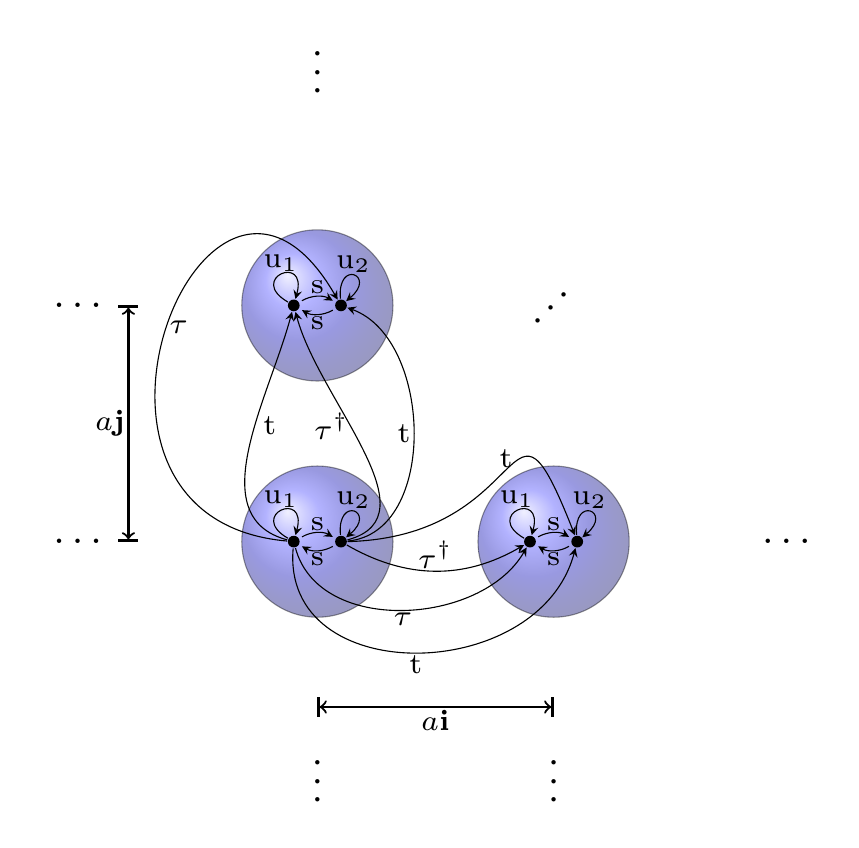
\begin{tikzpicture}[scale=3, every node/.style={scale=1.5}]
			\draw[shading=ball, opacity=0.4] (0,0) circle (3.2mm);
			\draw[shading=ball, opacity=0.4] (1,0) circle (3.2mm);
		\node[circle,fill=black, inner sep=1pt] (1) at (0.1,0){};
		\node[circle,fill=black, inner sep=1pt] (2) at (-0.1,0){};
		\node[circle,fill=black, inner sep=1pt] (3) at (1.1,0){};
		\node[circle,fill=black, inner sep=1pt] (4) at (0.9,0){};

			\draw[shading=ball, opacity=0.4] (0,1) circle (3.2mm);
		\node[circle,fill=black, inner sep=1pt] (5) at (0.1,1){};
		\node[circle,fill=black, inner sep=1pt] (6) at (-0.1,1){};
		\node (9) at (2,0) {\dots};
		\node (10) at (-1,0) {\dots};
		\node (12) at (-1,1) {\dots};
		\node[rotate=45] (11) at (1,1) {\dots};
		\node[rotate=90] (12) at (0,2) {\dots};
		\node[rotate=90] (14) at (0,-1) {\dots};
		\node[rotate=90] (15) at (1,-1) {\dots};
		\draw[->,>=stealth,shorten <=1pt,shorten >=1pt] (2) edge [bend left] node[midway, above, yshift=-1mm] {\scriptsize s} (1);
		\draw[->,>=stealth,shorten <=1pt,shorten >=1pt] (1) edge [bend left] node[midway, below, yshift=1mm] {\scriptsize s} (2);
		\draw (2) edge [loop above,>=stealth, ->, min distance = 2mm, out=150] node [yshift=-1mm] {\scriptsize $\rm u_1$} (2);
		\draw (1) edge [loop above,>=stealth, ->, min distance = 1.7mm, out=95, in=40] node [yshift=-1mm] {\scriptsize u$_2$} (1);
		\draw (1) edge [loop above,>=stealth, ->, out=5, in=-20] node [left, xshift=1mm] {$\scriptstyle \rm t$} (5);
		\draw (1) edge [loop above,>=stealth, ->, out=15, in=-75] node [left, yshift = 2mm] {$\scriptstyle \tau^\dagger$} (6);
		\draw[->,>=stealth,shorten <=1pt,shorten >=1pt] (6) edge [bend left] node[midway, above, yshift=-1mm] {\scriptsize s} (5);
		\draw[->,>=stealth,shorten <=1pt,shorten >=1pt] (5) edge [bend left] node[midway, below,yshift=1mm] {\scriptsize s} (6);
		\draw (6) edge [loop above,>=stealth, ->, min distance = 2mm, out=150] node [yshift=-1mm] {\scriptsize u$_1$} (6);
		\draw (5) edge [loop above,>=stealth, ->, min distance = 1.7mm, out=95, in=40] node [yshift=-1mm] {\scriptsize u$_2$} (5);
		\draw (2) edge [loop above,>=stealth, ->, out=175, in=120, min distance=11mm] node [right, xshift=-1mm] {$\scriptstyle \tau$}(5);
		\draw (2) edge [loop above,>=stealth, ->, out=165, in=-105] node [right, yshift = 2mm]{\scriptsize t} (6);

		\draw[->,>=stealth,shorten <=1pt,shorten >=1pt] (4) edge [bend left] node[midway, above, yshift=-1mm] {\scriptsize s} (3);
		\draw[->,>=stealth,shorten <=1pt,shorten >=1pt] (3) edge [bend left] node[midway, below,yshift=1mm] {\scriptsize s} (4);
		\draw (4) edge [loop above,>=stealth, ->, min distance = 2mm, out=150] node [yshift=-1mm] {\scriptsize u$_1$} (4);
		\draw (3) edge [loop above,>=stealth, ->, min distance = 1.7mm, out=95, in=40] node [yshift=-1mm] {\scriptsize u$_2$} (3);

		\draw (2) edge [loop above,>=stealth, ->, out=-75, in=-120] node [below, yshift=1mm] {$\scriptstyle \tau$}(4);
		\draw (2) edge [loop above,>=stealth, ->, out=-95, in=-105, min distance = 6mm] node [below, yshift = 1mm]{\scriptsize t} (3);
		\draw (1) edge [bend right,>=stealth, ->, out=0, in=110, min distance = 8mm] node [above, yshift=-1mm] {$\scriptstyle \rm t$} (3);
		\draw (1) edge [bend left,>=stealth, ->, out=-30, in=210] node [above, yshift = -1mm] {$\scriptstyle {\tau}^\dagger$} (4);
		\draw[|<->|, thick] (0,-0.7) -- (1,-0.7) node[below, midway, yshift=1mm] {$\scriptstyle a\bf i$};
		\draw[|<->|, thick] (-0.8,0) -- (-0.8,1) node[left, midway, xshift=1mm] {$\scriptstyle a\bf j$};

	\end{tikzpicture}
\end{center}
\caption{\footnotesize Depiction of an infinite square mesh of atoms in two bands separated by $a$ showing the self energy u, the band gap energy s, the hopping ground state energy t and hopping band energy $\tau$.}\label{squarechain}
\end{figure}
\par	In the two band model, the interaction between these two bands must also be considered. This means the potential of an electron associated with the onsite atom is now more complicated. Similarly, hopping to another atomic site is more complicated since there are multiple bands to hop to. Figure \ref{squarechain} indicates the origin of these terms. Nearest neighbour interactions are the only terms considered in this example, in this case Equations \eqref{t}, \eqref{u} may be used which are the $2\times2$ matrices
	\begin{equation}
		\bf u=\begin{pmatrix} \rm u_1&s\\s&\rm u_2 \end{pmatrix} \qquad,\qquad \qquad \bf t=\begin{pmatrix} \rm t&\tau\\\tau^\dagger&\rm t\end{pmatrix}
	\end{equation}
	The self-energy is ${\rm u}_i$ for $i \in [1,2] \in \mathbb{Z}$ the two bands, and $s$ is the energy required to raise (lower) an electron to a more (less) excited state on the same atom. t is the energy required to hop to an equivalent excited state on a neighbouring atom, and $\tau$ is the hopping to a differently excited state on a neighbouring atom. In real space, the Hamiltonian is now block diagonalised
	\begin{equation}
	\bf	H = \begin{pmatrix} \ddots&\ddots& \bf 0&\bf 0\\\ddots&\bf u &\bf t&\bf 0\\\bf 0&\bf t^\dagger&\bf u&\ddots\\\bf 0&\bf 0&\ddots&\ddots\end{pmatrix}
	\end{equation}
	The reciprocal space Hamiltonian $\mathcal{H}=\langle {\bf k}|\bf H|{\bf \acute{k}} \rangle$ is obtained using Equation \eqref{kkk} 

	\begin{equation}
		\mathcal{H} = \begin{pmatrix} \ddots&\ddots& \bf 0&\bf 0\\\ddots&\bf u &{\bf t}\sum_{\bf d} e^{i\bf k \cdot d}&\bf 0\\\bf 0&{\bf t}^\dagger\sum_{\bf d} e^{-i\bf k \cdot d}&\bf u&\ddots\\\bf 0&\bf 0&\ddots&\ddots\end{pmatrix}
	\end{equation}

	In the case of the square lattice the primitive position vectors are ${\bf a}_1 = a(0,1)$, \quad ${\bf a}_2 = a(1,0)$ and ${\bf d}$ is the set of nearest neighbours $\pm {\bf a}_1, \pm {\bf a}_2$.
Summing all elements and scaling as $1/N$ yields
	\begin{equation}\label{H_0}
		\mathcal{H}(\bf k) = \mathcal{H}_{n-1,n} + \mathcal{H}_{n,n} + \mathcal{H}_{n+1,n}
	\end{equation}

	The assumption is made that the leading diagonal of $\bf t$ is real, so for a two band system
	Since Eq.\eqref{H_0} is also a matrix expression, the band energies $\varepsilon(\bf k)$ are the eigenvalues of this equation
	\begin{equation}
		\rm det \begin{pmatrix} \rm u_1+2t\cos \left(\bf k_\parallel{\mathnormal a} \right)-\varepsilon(\bf k) &s+2\tau
			\cos \left( {\bf k_\parallel}a \right) \\ s+2
			\tau^\dagger\cos \left({\bf k_\parallel}a \right) &\rm u_2+2t\cos \left( \bf k_\parallel {\mathnormal a}
\right)-\varepsilon(\bf k) \end{pmatrix} =0
	\end{equation}
	thus
	% \begin{multline}
	% 	\varepsilon(\bf k) =\rm u+\left(t_{{11}}+t_{{22}}\right)\left(\cos \left( k_x{\mathnormal a} \right)+ \cos \left( k_z{\mathnormal a} \right) \right)
 % \pm \\\sqrt{\rm { \left(\left({t_{{11}}} 
 % -{t_{{22}}}\right)^2+4 t_{{12}}t_{{21}}\right)\left(\cos \left( k_x{\mathnormal a} \right) +\cos \left( k_z{\mathnormal a} \right)\right)^2
 % +2{\mathnormal s}\left(t_{{12}}+t_{{21}}\right)
 % \left(\cos \left( k_x\mathnormal a \right)+\cos \left( k_z\mathnormal a \right)\right) +{\mathnormal s}^{2}}}
	% \end{multline}

	\begin{multline}
		\varepsilon({\bf k}) =\frac{1}{2}(\rm u_1+u_2)+2t\left(\cos \left( k_x{\mathnormal a} \right)+ \cos \left( k_z{\mathnormal a} \right) \right)
 \pm \\\sqrt{\rm { 4 \tau\tau^\dagger\left(\cos \left( k_x{\mathnormal a} \right) +\cos \left( k_z{\mathnormal a} \right)\right)^2
 +2{\mathnormal s}\left(\tau+\tau^\dagger\right)
 \left(\cos \left( k_x\mathnormal a \right)+\cos \left( k_z\mathnormal a \right)\right) +{\mathnormal s}^{2}+\frac{1}{4}\left(u_1 -u_2\right)^2}}
	\end{multline}
	Where upon switching off $s, \tau$ and making u$_1 = $u$_2$ yields the one-band case, as expected.
	

	\subsection{Surface Green's function}
	The tight binding method is useful for describing infinite crystals, but in the study of mutlilayer systems, edge effects (surfaces) must be appropriately considered.
	\gls{sgf}'s allow this to be possible and are an extension of the tight binding framework.
	Two methods for determining closed-form \gls{sgf} will now be given. The first method, the Kalkstein \& Soven method is for historical purposes and has little practical significance as it fails to determine \gls{sgf} for more than one band. It is derived with the \gls{sc} lattice in consideration. The second method, the M\"{o}bius transformation method is far more general and very powerful.
	\subsubsection{Kalkstein \& Soven Method}\label{k_s}
	Initially, a perfect infinite \gls{sc} crystal is considered and separated artificially into two semi-infinite crystals along some imaginary cleavage plane in an arbitrary crystallographic direction\textcolor{blue}{\textsuperscript{ \cite{phan,KS}}}.
The perfect crystal has Hamiltonian $H^0$ and Green's function $G^0 (\varepsilon-H^0+i\delta)=1$ where $\delta$ is a positive infinitesimal contribution to the energy. The cleaved crystal has Hamiltonian $H$ and Green's function $G(\varepsilon-H+i\delta)=1$ where $H = H^0 + V$ and $V$ is the potential arising due to the perturbation of the introduced surface. Thus $G(\varepsilon-H^0-V+i\delta)=1$ which implies $G(\varepsilon-H^0-V+i\delta)G^0=G^0$. Since $G^0$ is commutative the reformulation is possible $(\varepsilon-H^0+i\delta)G^0=1$. Making this substitution above yields $G(1-VG^0)=G^0$ and so the familiar Dyson's equation follows; 
\begin{equation}\label{dyson}
G=G^0+GVG^0 
\end{equation}
The coordinates of any atomic site in three dimensions are given by ${\bf{R}} = n_1{\bf{a_1}}+n_2{\bf{a_2}}+n_3{\bf{a_3}}$ where $\bf a_1, a_2, a_3$ are vectors in the $x, y,z$-directions respectively. In this formalism however, the crystal is no longer infinite perpendicular to plane, thus the alternative basis ${\bf R} = n{\bf a}+{\bf R_\parallel}$ is used where $n=n_1$ and $\bf a=a_1$ is a vector perpendicular to the cleaved surface and $\bf R_\parallel$ refers to those sites parallel to the surface (surface plane).
The representation in the surface plane is Bloch-like so the transform to the momentum space basis is as follows
\begin{equation}
|n,{\bf k_\parallel} \rangle = \frac{1}{\sqrt{N_\parallel}}\sum_{\bf R_\parallel} |n{\bf a} + {\bf R_\parallel}\rangle e^{i\bf k_\parallel\cdot R_\parallel}
\end{equation}
The representation perpendicular to the surface plane is finite and thus the mixed Bloch-Wannier form is used
\begin{equation}
	|{\bf k} \rangle =|{\bf k_\perp,k_\parallel}\rangle = \frac{1}{\sqrt{N_\perp}}\sum_n |n{\bf a,k_\parallel}\rangle e^{in{\rm{k}}_\perp a}
\end{equation}
By the tight binding model, the Green's function of the unperturbed crystal is
\begin{equation}
\langle {\bf k}|G^0|{\bf \acute{k}} \rangle = \frac{\delta_{\bf k-\acute{k}}}{\varepsilon-E^0 ({\bf k}) +i\delta}
\end{equation}
Where $\delta_{\bf k-\acute{k}}$ is the Dirac-Delta function which is non-zero only for the very small range of values around $\bf k = \acute{k}$. Here the result $\langle {\bf k}|H^0|{\bf \acute{k}} \rangle = E^0 ({\bf k}) $ has been used, where
\begin{equation}
	E^0 ({\bf k})={\rm{u}}+2{\rm{t}}[\cos({\rm{k}}_\perp a)+f({\bf k_\parallel})]
\end{equation}
where
\begin{equation}\label{disp}
	f({\bf k_\parallel}) = \cos({\rm{k}}_y a)+\cos({\rm{k}}_z a)
\end{equation}
in the simple cubic case, as described here. Therefore
\begin{equation}
	G^0(n - \acute{n}) = \left[ \frac{1}{\sqrt{N_\perp}}\sum_{\acute{n}} \langle{\bf k_\parallel}|e^{-i\acute{n}{\rm{k}}_\perp a}\right]\cdot \frac{1}{\varepsilon-E^0 ({\bf k}) +i\delta} \cdot \left[ \frac{1}{\sqrt{N_\perp}}\sum_n |{\bf k_\parallel}\rangle e^{in{\rm{k}}_\perp a}\right]
\end{equation}
which yields the Green's function for each layer $|n| = (n-\acute{n})$,
\begin{equation}
	G^0 (n) = \frac{1}{N_\perp}\sum_{{\rm{k}}_\perp} \frac{e^{i|n|{\rm{k}}_\perp a}}{\varepsilon-E^0 ({\bf k}) +i\delta} \quad .
\end{equation}
This is solved most conveniently by converting the summation to an integral and solving by contour integration.
\begin{equation}
	G^0 (n) = \frac{a}{2\pi}\int_{-\frac{\pi}{a}}^{\frac{\pi}{a}} {d{\rm{k}}_\perp} \frac{e^{i|n|{\rm{k}}_\perp a}}{\varepsilon-E^0 ({\bf k}) +i\delta}
\end{equation}
where the range of integration is over the first Brillouin zone. Putting $\omega = \varepsilon -{\rm u} -2{\rm t}f({\bf k_\parallel})$ yields
\begin{equation}
	G^0 (n) = \frac{a}{2\pi}\int_{-\frac{\pi}{a}}^{\frac{\pi}{a}} {d{\rm k}_\perp} \frac{e^{i|n|{\rm k}_\perp a}}{\omega +i\delta - 2{\rm t}\cos({\rm k}_\perp a)} .
\end{equation}
The substitution $z=e^{i{\rm k}_\perp a}$ is made, so that $\cos({\rm k}_\perp a) = \frac{1}{2}\big(e^{i{\rm k}_\perp a}+e^{-i{\rm k}_\perp a}\big)= \frac{1}{2}\big(z +\frac{1}{z}\big)$.
\\Also $\frac{dz}{d{\rm k}_\perp}=iaz , \quad d{\rm k}_\perp =\frac{dz}{iaz},$ thus integrating over the unit circle $C$ yields
\begin{equation}
	G^0 (n) = \frac{a}{2\pi}\oint_C \frac{dz}{iaz}\cdot \frac{z^{|n|}}{\omega +i\delta - {\rm t}z-{\rm t}z^{-1}} 
\end{equation}
now letting $\delta \longrightarrow 0$, and rearranging
\begin{equation}
	G^0 (n) = \frac{i}{2\pi}\oint_C dz\frac{z^{|n|}}{{\rm t}(z^2 -\omega z/{\rm t}+1)} 
\end{equation}
the denominator of the integrand is equivalent to
\begin{equation}
	\left(z-\frac{\omega-\sqrt{\omega^2 -4{\rm t}^2}}{2{\rm t}} \right)\left(z-\frac{\omega+\sqrt{\omega^2 -4{\rm t}^2}}{2{\rm t}} \right)
\end{equation}
thus the singularities are at $z=\frac{\omega-\sqrt{\omega^2 -4{\rm t}^2}}{2{\rm t}}$ and $z=\frac{\omega+\sqrt{\omega^2 -4{\rm t}^2}}{2{\rm t}}$ but only one of these is within the unit circle, and this depends on the sign and ratio of certain quantities. Thus there is one residue, and when $\omega > 0, \quad (\omega^2 -4{\rm t}^2 \geq 0)$ it is at the former, thus
\begin{equation}
	G^0 (n) = \frac{i}{2\pi}\left[\frac{2\pi i}{\rm t} \cdot \frac{z^{|n|}}{z-\frac{\omega+\sqrt{\omega^2 -4{\rm t}^2}}{2{\rm t}}}\right]\Bigg|_{z = \frac{\omega-\sqrt{\omega^2-4{\rm t}^2}}{2{\rm t}}}
\end{equation}
\begin{equation}
G^0 (n) = \frac{1}{\alpha}\left( \frac{\omega-\alpha}{2\rm t}\right)^{|n|} 
\end{equation}
where $ \alpha = \sqrt{\omega^2-4{\rm t}^2} $.
When $\omega < 0, \quad (\omega^2 -4{\rm t}^2 \geq 0)$ the residue is at $z=(\omega+\sqrt{\omega^2 -4{\rm t}^2})/2\rm t$, thus
\begin{equation}
G^0 (n) = \frac{1}{-\alpha}\left( \frac{\omega+\alpha}{2\rm t}\right)^{|n|}  .
\end{equation}
These two expressions can be put more succinctly as follows
\begin{equation}
	G^0 (n) = \frac{1}{\alpha \rm{sign}(\omega)}\left( \frac{\omega-\alpha \rm{sign}(\omega)}{2\rm t}\right)^{|n|}\label{alpha}
\end{equation}
where $|n|$ is used since symmetry is required on either side of the cleavage plane.
The final situation to consider is $\omega^2 -4{\rm t}^2 < 0$, in which case the residue is at $z=(\omega+\sqrt{\omega^2 -4{\rm t}^2})/2\rm t$, or $z=(\omega +i\sqrt{4{\rm t}^2-\omega^2})/2\rm t$. Thus
\begin{equation}\label{mu}
G^0 (n) = \frac{i}{\mu}\left( \frac{\omega+i\mu}{2\rm t}\right)^{|n|} 
\end{equation}
where 
\begin{equation}
	\mu = \sqrt{4{\rm t}^2-\omega^2} .
\end{equation}
Returning to the Dyson's equation \eqref{dyson}, which in this representation reduces to the set of equations
\begin{equation}\label{Gsum}
G(m,n)=G^0(m,n)+\sum_{p,q} G^0 (m,p)V(p,q)G(q,n)
\end{equation}
but $V(m,n)$ is only non-zero for sites on opposing surface planes so $p$ and $q$ only yield non-zero values when they are equal to $-1$ or $0$ and not equal to each other. Thus in full
\begin{multline}
G(m,n)=G^0(m,n)+G^0 (m,-1)V(-1,0)G(0,n)\\ +G^0 (m,0)V(0,-1)G(-1,n)
\end{multline} 
but $G(-1,n)=0$ for $n \geq 0 $ as these refer to sites on different crystals. Thus
\begin{equation}\label{GGG}
G(m,n)=G^0(m,n)+G^0 (m,-1)V(-1,0)G(0,n)
\end{equation}
and $V(-1,0)$ must be equal to $-\rm t$, since $V$ exists to cancel the interactions between the exposed surfaces. Also since $G^0$ depends only upon the difference $m-n$ since it is the Green's function for the perfect crystal\textcolor{blue}{\textsuperscript{\cite{KS}}},
\begin{equation}
	G(m,n)=G^0(m-n)-{\rm t} G^0 (m+1)G(0,n)
\end{equation}
Thus the semi-infinite Green's function for the cleaved crystal is
\begin{equation}
	G(m,m)=G^0(0)-{\rm t} G^0 (m+1)G(0,m)
\end{equation}
where
\begin{equation}
	G(0,m)=G^0(-m)-{\rm t} G^0 (1)G(0,m)
\end{equation}
thus
\begin{equation}
	\left[1+ {\rm t}G^0 (1)\right]G(0,m) =G^0 (-m)
\end{equation}
thus
\begin{equation}\label{G}
	G(m,m)=G^0(0)+\left[-{\rm t} G^0 (m+1)\right] G^0(-m)\left[1+ {\rm t}G^0 (1)\right]^{-1}
\end{equation}
\qquad \qquad \qquad for $m \geq 0$.
At this stage the Green's function may be elicited from equations \eqref{alpha} \& \eqref{mu}. Starting with equation \eqref{alpha}, i.e. the case $\omega^2-4{\rm t}^2>0$,  where here the substitution $\eta = \alpha \rm{sign}(\omega)$ is made
\begin{equation}
G(m,m)= \frac{1}{\eta}-\frac{\rm t}{\eta^2}\left(\frac{\omega -\eta}{2\rm t}\right)^{|2m+1|}\left[1+\frac{1}{\eta}\left(\frac{\omega -\eta}{2}\right)\right]^{-1}
\end{equation}
thus
\begin{equation}
G(m,m)= \frac{1}{\eta}+\left[ \frac{1}{\eta}\left(\frac{\eta -\omega}{2}\right)\left(\frac{\omega -\eta}{2\rm t}\right)^{2|m|}\right]\left[\frac{\eta+\omega}{2}\right]^{-1}
\end{equation}
\\
thus
\begin{equation}
	G(m,m)= \frac{1}{\eta}\left[1+\left(\frac{\omega -\eta}{2\rm t}\right)^{2|m|}\frac{\left(\eta-\omega\right)}{\left(\eta+\omega\right)}\right] , \qquad \omega^2 -4{\rm t}^2>0
\end{equation}
\\
And now the case $\omega^2-4{\rm t}^2<0$, obtained by substituting equation \eqref{mu} into equation \eqref{G}
\begin{equation}
G(m,m)= \frac{i}{\mu}+\left[ -\frac{i\rm t}{\mu}\left(\frac{\omega +i\mu}{2\rm t}\right)^{|m+1|}\right]\left[\frac{i}{\mu}\left(\frac{\omega +i\mu}{2\rm t}\right)^{|m|}\right]\left[1+\frac{i\rm t}{\mu}\left(\frac{\omega +i\mu}{2\rm t}\right)\right]^{-1}
\end{equation}
thus
\begin{equation}
G(m,m)= \frac{i}{\mu}+\left[ -\frac{i}{\mu}\left(\frac{\omega+i\mu}{2}\right)\left(\frac{\omega +i\mu}{2\rm t}\right)^{2|m|}\right]\left[\frac{-i\mu +\omega}{2}\right]^{-1}
\end{equation}
thus
\begin{equation}
	G(m,m)= \frac{i}{\mu}\left[1+\left(\frac{\omega +i\mu}{2\rm t}\right)^{2|m|}\frac{\left(\mu-i\omega\right)}{\left(\mu+i\omega\right)}\right], \qquad \omega^2-4{\rm t}^2<0
\end{equation}
\\
Throughout the remainder of this communication the convention $ G(0,0)\equiv {\rm{g_0}}$ is used.
\\[2mm]To demonstrate one of the potential uses of \gls{sgf}'s, the \acrfull{ldos} will be calculated at different atomic layers.
In the mixed representation, the \gls{ldos} is defined by
\begin{equation}\label{rho}
	\rho_m(\varepsilon)=\frac{-1}{\pi N_\parallel}\sum_{\bf k_\parallel} \Im\left\{ G(m,m,{\bf k_\parallel})\right\}\site{KS}.
\end{equation}
Eq. \eqref{rho} is calculated numerically by converting the summation into a double integral over the two dimensional Brillouin zone
\begin{equation}
	\rho_m(\varepsilon)=\frac{-a^2}{4\pi^3} \int_{-\frac{\pi}{a}}^{\frac{\pi}{a}}\int_{-\frac{\pi}{a}}^{\frac{\pi}{a}} d{\rm k}_y d{\rm k}_z  G(m,m,{\rm k}_y,{\rm k}_z).
\end{equation}
\begin{figure}[H]
	\centering
\begin{tikzpicture} 
	% \draw[black!50] (0,0)--(2.4in,1.8in);
	% \draw[black!50] (0,2.4in)--(2.4in,4.2in);
	% \draw[black!50] (3.4in,0)--(5.8in,1.8in);
	\begin{axis}[
			width = 3in,height=2.25in,
			axis line style=purple,
			axis y line*=left,
			legend style={xshift=0.2in,yshift=-0.5in, draw=none},
			axis x line*=bottom,
			title=\large Local Density of States (LDOS),
			title style={xshift = -5cm},
			xshift=3in,
			yshift=1.8in,
			% scaled y ticks = false,
			% ymin=0,
			% xmin=2,
			% xmax=51,
		]
		\addplot[purple, very thick] table [col sep=comma] {6th.txt};\addlegendentry{$n=6$}
	\end{axis}
	\begin{axis}[
			width = 3in,height=2.25in,
			legend style={xshift=1in,yshift=-1.3in, draw=none},
			axis line style=blue,
			axis y line*=left,
			axis x line*=bottom,
			xshift=2in,
			yshift=1.2in,
		]
		\addplot[blue, very thick] table [col sep=comma] {2nd.txt};\addlegendentry{$n=2$}
	\end{axis}
	\begin{axis}[
			width = 3in,height=2.25in,
			axis line style=red,
			axis y line*=left,
			legend style={xshift=1in,yshift=-1.3in, draw=none},
			axis x line*=bottom,
			xshift=1in,
			yshift=0.6in,
		]
		\addplot[red, very thick] table [col sep=comma] {1st.txt};\addlegendentry{$n=1$}
	\end{axis}
	\begin{axis}[
			width = 3in,height=2.25in,
			axis line style=blue!40!green,
			axis y line*=left,
			axis x line*=bottom,
			legend style={xshift=1in,yshift=-1.3in, draw=none},
			xlabel style={xshift=1.2in},
			xlabel=Energy $\varepsilon \quad (eV)$,
			ylabel style={xshift=1in},
			ylabel=\gls{ldos} $\rho \quad(eV^{-1}\si{\angstrom}^{-2})$,
		]
		\addplot[blue!40!green,very thick] table [col sep=comma] {0th.txt};\addlegendentry{$n=0$}
	\end{axis}

\end{tikzpicture}
\caption{\footnotesize \gls{ldos} with potential $u = 0eV$, ${\rm t} = 0.5eV$. The plots above are for atomic layers of various depth from the surface, $n$, with the surface layer $n=0$. Results calculated using C++98 with Clang compiler.}\label{LDOS}
\end{figure}
Figure \ref{LDOS} shows the calculated \gls{ldos} against energy for up to the sixth atomic plane. The following results are noted; the profile of the \gls{ldos} for larger $n$ heals very quickly to the bulk value, and has two distinct zones. 
\par The region $-2\rm t \leq \varepsilon \leq 2t$, the width of the allowed values of the in-plane element of the dispersion relation Eq. \eqref{disp}, is some periodic function that flattens out the larger the value $n$ chosen. This region is flat in the case of an infinite crystal. The region $\varepsilon<-2\rm t, \varepsilon>2t$ appears to be almost parabolic. The on-site energy $\rm u$ displaces the whole function along the $\varepsilon$ axis. The full width of the function is 12t, the width of the dispersion relation.
By definition, integrating the \gls{ldos} gives $1$.
	\subsubsection{Method of Adlayer}
	A simple method to gain \gls{sgf}'s for additional 'deposited' atomic planes is the so called 'Adlayer' method, which essentially connects the previous \gls{sgf} to the deposited \gls{sgf} through the Dyson's equation. It is an iterative equation depending only on the previous \gls{sgf} through each computation. To calculate this it can be noted that Equation \eqref{Gsum} is equally valid for matrices, and so Equation \eqref{GGG} is rewritten in this context to find ${\bf G}_{11}$, the first Green's function deposited on the substrate
	\begin{equation}\label{G11}
	{\bf G}_{11}^1={\bf G}_{11}^0+{\bf G}_{11}^1{\bf V}_{11}{\bf G}_{11}^0 +{\bf G}_{10}^1{\bf V}_{01}{\bf G}_{11}^0
\end{equation}
Using Equation \eqref{Gsum} to find ${\bf G}_{10}^1$
\begin{equation}\label{G10}
	{\bf G}_{10}^1={\bf G}_{11}^1{\bf V}_{10}{\bf G}_{00}^0
\end{equation}
since ${\bf V}_{00} = \bf 0$, ${\bf G}_{10}^0 = \bf 0$. Substituting Equation \eqref{G10} into Equation \eqref{G11} yields
	\begin{equation}
	{\bf G}_{11}^1={\bf G}_{11}^0+{\bf G}_{11}^1{\bf V}_{11}{\bf G}_{11}^0 +{\bf G}_{11}^1{\bf V}_{10}{\bf G}_{00}^0{\bf V}_{01}{\bf G}_{11}^0
\end{equation}
which can be manipulated to
	\begin{equation}
		({\bf G}_{11}^1)^{-1}{\bf G}_{11}^1=({\bf G}_{11}^1)^{-1}{\bf G}_{11}^0+({\bf G}_{11}^1)^{-1}{\bf G}_{11}^1{\bf V}_{11}{\bf G}_{11}^0 +({\bf G}_{11}^1)^{-1}{\bf G}_{11}^1{\bf V}_{10}{\bf G}_{00}^0{\bf V}_{01}{\bf G}_{11}^0
\end{equation}
which simplifies to 
	\begin{equation}
		{\bf I}=({\bf G}_{11}^1)^{-1}{\bf G}_{11}^0+{\bf V}_{11}{\bf G}_{11}^0 +{\bf V}_{10}{\bf G}_{00}^0{\bf V}_{01}{\bf G}_{11}^0
\end{equation}
which can be reordered to yield
	\begin{equation}
		{\bf I}=\left(({\bf G}_{11}^1)^{-1}+{\bf V}_{11} +{\bf V}_{10}{\bf G}_{00}^0{\bf V}_{01}\right){\bf G}_{11}^0
\end{equation}
thus
	\begin{equation}
		({\bf G}_{11}^0)^{-1}=({\bf G}_{11}^1)^{-1}+{\bf V}_{11} +{\bf V}_{10}{\bf G}_{00}^0{\bf V}_{01}
	\end{equation}
so upon reordering and taking appropriate inverses	
	\begin{equation}\label{adlayer_0}
		{\bf G}_{11}^1=\left(({\bf G}_{11}^0)^{-1}-{\bf V}_{11} -{\bf V}_{10}{\bf G}_{00}^0{\bf V}_{01}\right)^{-1}
	\end{equation}
	Now from the definition of Green's function, the term ${\bf G}_{11}^0 = (\bm\varepsilon)^{-1}$. ${\bf V}_{11} = \bf u$, where $\bf u$ is the potential of the adlayered plane, ${\bf V}_{10}=\bf t^\dagger$ is the hopping from the adlayer to the substrate and ${\bf V}_{01} = \bf t$ is the hopping from the substrate to the adlayer. Where the indices of the Green's functions are the same, this indicates they are \gls{sgf}'s and thus Equation \eqref{adlayer_0} can be presented as follows

\begin{equation}
	{\bf g}_1 = ({\bf v-t}^{\dag}{\bf g}_0{\bf t})^{-1}
\end{equation}
where $\bf v = \bm\varepsilon-u$. Repeating the adlayer process leads to the iterative formula
\begin{equation}\label{adlayer}
	\bf{g_{\rm n}} = (\bf{v}-\bf{t}^{\dag}\bf{g_{\rm n-1}t})^{\rm -1}
\end{equation}
an exact form of a closed-form \gls{sgf} in terms of ${\bf g}_0$. What makes Equation \eqref{adlayer} particularly interesting is the fact that different materials may be stacked upon each other without loss of accuracy. Thus it makes a good vehicle for studying multilayer systems.
	\subsubsection{M\"{o}bius Transformation method}
	The Kalkstein \& Soven method outlined in Subsection \ref{k_s} is one of the first closed-form Green's function formalisms derived, however it fails to describe the case when Green's functions are matrices. For any realistic calculations, this becomes a requirement. 
An alternative method known as the M\"{o}bius Transformation method, or the method of Umerski\textcolor{blue}{\textsuperscript{\cite{AU_SGF}}} is used in these cases.
\\\par As in Section \ref{k_s}, the formalism required is that of a crystal, infinite along two axes (in plane) and finite in the growth direction (out-of-plane). Due to the structure of the crystal here, the standard tight-binding model in three dimensions outlined in Section \ref{tb} does not apply.
Instead, the Hamiltonian must be diagonalised in-plane, but unless the crystal is \gls{sc}, in general more than one basis atom must be considered to cater for the principle layers, such that there is translational symmetry in the growth direction, and so that interactions between these layers are accounted for.
\\\par Thus the location of any atomic site is given by ${\bf R} = {\bf R}_\parallel + {\bf R}_\perp +{\bf s}_i$, where ${\bf R}_\parallel = n_1{\bf a}_1+n_2{\bf a}_2$ represents the sites on the plane parallel to the surface per basis atom, with integers $n_1,n_2$ and ${\bf a}_1,{\bf a}_2$ are the primitive translation vectors. The vector ${\bf R}_\perp = \rm n\bf a$ represents the sites along the growth direction, generally the $y$-axis (${\bf k}_y$-axis in reciprocal space) such that ${\bf a} = a(0,1,0)$, n is the nth plane from the \gls{sgf} and $a$ is the distance between planes.
${\bf s}_i$ is the location of the basis atoms. For example, \gls{bcc} has the two basis atoms at ${\bf s}_1 = (0,0,0), 	{\bf s}_2 = \frac{a}{2}(1,1,1)$, the two sites in a primitive (symmetrically irreducible) cell.
	\tikzset{external/export next=false}
	\begin{figure}[H]
		\begin{center}
	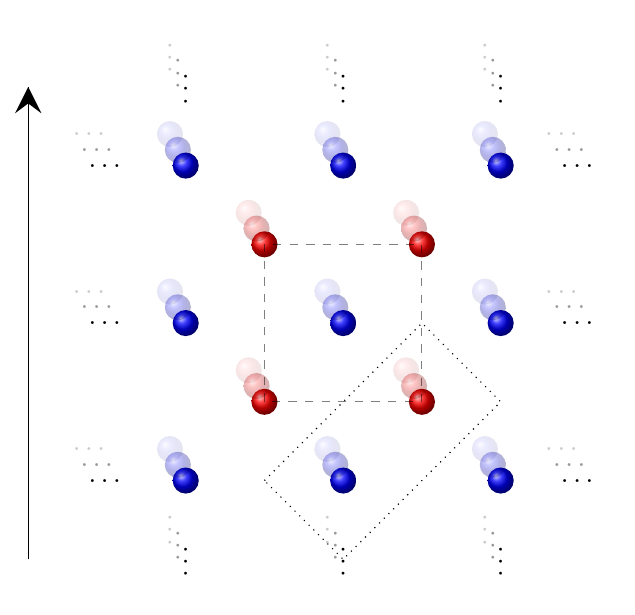
\begin{tikzpicture}
		\foreach \x in {1,3,5} {
			\foreach \y in {1,3,5} {
				\node at (\x,\y) [circle, shading=ball]{};
				\node at (\x-0.1, {\y+0.2}) [circle, shading=ball, opacity = 0.3]{};
				\node at (\x-0.2, {\y+0.4}) [circle, shading=ball, opacity = 0.1]{};
			}
		}
		\foreach \x in {2,4}{
			\foreach \y in {2,4}{
				\node at (\x,\y) [circle, shading=ball, ball color=red]{};
				\node at (\x-0.1, {\y+0.2}) [circle, shading=ball, ball color=red, opacity = 0.3]{};
				\node at (\x-0.2, {\y+0.4}) [circle, shading=ball, ball color=red, opacity = 0.1]{};
			}
		}
		\foreach \x in {1,3,5} {
			\node at (0,\x) {\dots};
			\node at (6,\x) {\dots};
			\node at (-0.1,\x+0.2) [opacity=0.4] {\dots};
			\node at (5.9,\x+0.2) [opacity=0.4] {\dots};
			\node at (-0.2,\x+0.4) [opacity=0.2] {\dots};
			\node at (5.8,\x+0.4) [opacity=0.2] {\dots};
		}
		\foreach \x in {1,3,5} {
			\node at (\x, 0) [rotate=90] {\dots};
			\node at (\x, 6) [rotate=90] {\dots};
			\node at (\x-0.1, 0.2) [rotate=90,opacity=0.4] {\dots};
			\node at (\x-0.1, 6.2) [rotate=90,opacity=0.4] {\dots};
			\node at (\x-0.2, 0.4) [rotate=90,opacity=0.2] {\dots};
			\node at (\x-0.2, 6.4) [rotate=90,opacity=0.2] {\dots};
		}
		\draw[dashed, opacity = 0.5] (2,2) -- (2,4) -- (4,4) -- (4,2) -- cycle;
		\draw[dotted] (2,1) -- (4,3) -- (5,2) -- (3,0) -- cycle;
		\draw [decoration={markings,mark=at position 1 with
    {\arrow[scale=3,>=stealth]{>}}},postaction={decorate}](-1,0) -- (-1, 6);

	\end{tikzpicture}
\end{center}
\caption{\footnotesize The above figure shows a \gls{bcc} lattice with atomic planes stacked in the growth direction. The dashed region indicates the first Brillouin zone centred on the site at $(0,0,0)$, and the dotted region shows a primitive cell enclosing sites $a(0,-1,0)$ and $\frac{a}{2}(1,-1,1)$. It can be observed that the primitive cells tesselate completely, which forms part of their definition.}
\end{figure}
The representation in $k$-space is thus
	\begin{equation}
		|{\bf k}_\parallel, {\bf k}_\perp, {\bf s}_i\rangle = \frac{1}{\sqrt{N_\parallel}}\sum_{\bf R_\parallel = -\infty}^\infty e^{i{\bf k}_\parallel\cdot {\bf R}_\parallel} |{\bf R}_\parallel,{\bf R}_\perp, {\bf s}_i \rangle
	\end{equation}
	Thus the diagonalised Hamiltonian can be given by 
	\begin{equation}\label{multibasis}
		\langle{\bf k}_\parallel, {\bf k}_\perp, {\bf s}_i|{\bf H}|{\bf \acute{k}}_\parallel, {\bf \acute{k}}_\perp, {\bf s}_j\rangle = \frac{1}{N_\parallel}\sum_{\bf R_\parallel \acute{R}_\parallel}  e^{i({\bf \acute{k}}_\parallel\cdot {\bf \acute{R}}_\parallel-{\bf k}_\parallel\cdot {\bf R}_\parallel)} \langle{\bf R}_\parallel,{\bf R}_\perp, {\bf s}_i|{\bf H}|{\bf \acute{R}}_\parallel,{\bf \acute{R}}_\perp, {\bf s}_j \rangle
	\end{equation}
	An example is now given, the \gls{bcc} structure.
	In this case, the basis atoms are located at ${\bf s}_1=(0,0,0), \, {\bf s}_2=\frac{a}{2}(1,1,1)$.
	The principle lattice vectors are ${\bf a}_1 = a(1,0,0), \, {\bf a}_2 = a(0,0,1), \, {\bf a}_3 = a(0,1,0)$,
	with ${\bf R}_\parallel = n_1{\bf a}_1 + n_2{\bf a}_2, \, {\bf R}_\perp = n_3 {\bf a}_3$.
	The potential of the onsite element of the first basis atom at ${\bf s}_1$ is ${\bf u}_1$ and the potential of the onsite element of the second basis atom at ${\bf s}_2$ is ${\bf u}_2$,
	where the bold typeface of these potentials indicates they are themselves matrices in multiband models.
	In this example, offsite terms up to second nearest neighbours are considered, where the first nearest neighbours have potential ${\bf t}_1$, and the second nearest neighbours have potential ${\bf t}_2$.
	Using Equation \eqref{multibasis} in conjunction with Equation \eqref{kk} yields
	\begin{equation}
		equation required here
	\end{equation}
	% In this case, considering nearest neighbours and next nearest neighbours, the only non-zero elements of the in-plane Hamiltonian are
	% \begin{equation}
	% 	\langle{\bf R}_\parallel,{\bf R}_\perp, {\bf s}|{\bf H}|{\bf R}_\parallel,{\bf R}_\perp, {\bf s} \rangle = \bm \mu
	% \end{equation}
	% \begin{equation}
	% 	\langle{\bf R}_\parallel,{\bf R}_\perp, {\bf s}|{\bf H}|{\bf R}_\parallel \pm {\bf d},{\bf R}_\perp, {\bf s} \rangle = \bf t
	% \end{equation} 
	% where $\bf d$ is the set of nearest neighbours in $\bf R_\parallel$ (which makes them next nearest neighbours in the \gls{bcc} structure.
	% \begin{equation}
	% 	\langle{\bf R}_\parallel,{\bf R}_\perp, {\bf s}|{\bf H}|{\bf R}_\parallel,{\bf R}_\perp+\bf a, {\bf s} \rangle = \bf t
	% \end{equation}
	% \begin{equation}
	% 	\langle{\bf R}_\parallel,{\bf R}_\perp, {\bf s}|{\bf H}|{\bf R}_\parallel,{\bf R}_\perp-\bf a, {\bf s} \rangle = \bf t^\dagger
	% \end{equation}
	% \begin{equation}\label{l}
	% 	\langle{\bf R}_\parallel,{\bf R}_\perp, {\bf s}_1|{\bf H}|{\bf R}_\parallel+{\bf c},{\bf R}_\perp, {\bf s}_2 \rangle = \bm l
	% \end{equation}
	% \begin{equation}\label{ldagg}
	% 	\langle{\bf R}_\parallel,{\bf R}_\perp, {\bf s}_1|{\bf H}|{\bf R}_\parallel+{\bf c},{\bf R}_\perp-{\bf a}, {\bf s}_2 \rangle = \bm{l}^\dagger
	% \end{equation}
	% where $\bf c$ is the set of vectors ${\bf 0}, a(-1,0), a(-1,-1), a(0,-1)$ such that Equations \eqref{l}, \eqref{ldagg} account for the four nearest neighbours in front, $\bm l$, and the four nearest neighbours behind, $\bm l^\dagger$.
	Thus the Hamiltonian describing potentials along atomic layers is given by
	\begin{equation}
	\bf	H = \begin{pmatrix} \bf u&\bf t& \bf 0&\bf 0\\\bf t^\dagger&\bf u &\ddots&\bf 0\\\bf 0&\ddots&\ddots&\bf t\\\bf 0&\bf 0&\bf t^\dagger&\bf u\end{pmatrix}
	\end{equation}
	where 
	\begin{equation}
		{\bf u} = \bm \mu + 2{\bf t}\left(\cos\left(k_x a\right)+\cos\left(k_z a\right)\right) + 4\left(\bm l + \bm l^\dagger\right)\cos\left(\frac{k_xa}{2}\right)\cos\left(\frac{k_za}{2}\right)\,.
	\end{equation}
	This ends the example.
	\\[2mm] The definition of an $N$-dimensional M\"{o}bius transformation is as follows, let
\begin{equation}
\bf{A} = \begin{pmatrix} \bf{a}&\bf{b}\\ \bf{c}&\bf{d} \end{pmatrix}
\end{equation}
Where $\bf{A}$ is a $2N \times 2N$ matrix, and $\bf{a}, \bf{b}, \bf{c}, \bf{d}, \bf{z}$ are $N \times N$ matrices, then
\begin{equation}\label{LHMT}
\bf{A \bullet z} = (\bf{az} + \bf{b})(\bf{cz} + \bf{d})^{\rm -1}
\end{equation}
is the left hand M\"{o}bius transformation of $\bf z$ by $\bf A$.
This leads to the following result, derived from the Dyson equation
\begin{equation}
	{\bf g}_{{\rm n}+1} = {\bf X}\bullet {\bf g}_{\rm n}
\end{equation}
where
\begin{equation}\label{X}
	\bf{X} = \begin{pmatrix} \bf0&\bf{t}^{\rm{-1}}\\-\bf{t}^{\rm{\dag}}&\bf{vt}^{\rm{-1}} \end{pmatrix}
\end{equation}
Here, each element is an $N \times N$ matrix and $\bf{0}$ is a matrix of zeroes. The formalism here assumes a psuedo one-dimensional crystal grown along an arbitrary axis with ${\bf v} = \bm\varepsilon - {\bf u}$. Equation \eqref{X} in its present form and the results that follow are defined for left hand surfaces. For right hand surfaces, values $\bf{t}$ and $\bf{t}^{\rm{\dag}}$ must be interchanged.
To generalise to a three-dimensional crystal, an alternative basis must be used such as that defined at the beginning of this subsection.

% \begin{equation}\label{disp}
% 	\bf{v} = \varepsilon . \bf{I} - \bf{u} - \rm2\bf{t}\cos({\bf{k_\parallel}}\mathnormal a)
% \end{equation}	

	% Where $\bf{u}$ is the on-site energy of each site and $a$ is the lattice constant. 
It can be shown that Equation \eqref{LHMT} is associative with respect to multiplication. A consequence of this is that 
\begin{equation}
\bf A\bullet(B\bullet z) = (AB)\bullet z
\end{equation}
utilising this result and iterating Equation \eqref{adlayer}, it can be shown that
\begin{equation}\label{bigG}
	{\bf g}_{\rm n} = ({\bf X})^{\rm n}\bullet {\bf g}_0
\end{equation}
Equation \eqref{bigG} can be expressed as 
\begin{equation}\label{frac}
	{\bf g}_{\rm n} = ({\bf O}\bm\Lambda^{\rm n}{\bf O}^{-1})\bullet {\bf g}_0
\end{equation}
Here ${\bf O}$ is the matrix of eigenvectors of ${\bf X}$, arranged into columns with associated eigenvalues $\lambda$ ordered in terms of their magnitudes as follows
\begin{equation}
	| {\lambda}_1 | \leq | {\lambda}_2 | \leq \ldots \leq | {\lambda}_{2N} |
\end{equation}
$\bm \Lambda$ is the diagonal eigenvalue matrix
\begin{equation}
	\bm \Lambda \equiv {\rm diag}(\lambda_1,\lambda_2,\dots,\lambda_{2N})
\end{equation}
such that 
	\begin{equation}
		{\bf O}^{-1} {\bf X}{\bf O} = \bm \Lambda
	\end{equation}
	Equation \eqref{frac} has the remarkable property of demonstrating the existence of interatomic \gls{sgf} representations due to the continuity at non-integer n.
	\par To obtain the closed form \gls{sgf} ${\bf g}_0$ for semi-infinite systems, the ordering of the eigenvalues must be more precise\site{rev3}. To do this, a small positive imaginary contribution is made to the energy, such that $\varepsilon \longrightarrow \varepsilon+i\delta$ but to enforce n $\rightarrow \infty$ before $\delta \rightarrow 0$. This has the effect of shifting pairs of eigenvalues on the unit circle such that one moves just inside the circle and the other just outside. The former are in $\bm \Lambda_1$ and the latter are in $\bm \Lambda_2$, such that as $\rm n\rightarrow\infty$, \quad $\bm\Lambda_1^{\rm n}, \bm\Lambda_2^{-\rm n}\rightarrow 0$, where
	\begin{equation}
		\bm \Lambda = \begin{pmatrix} \bm \Lambda_1&\bf 0\\\bf 0&\bm \Lambda_2 \end{pmatrix}
	\end{equation}
	The linearly transformed \gls{sgf} is introduced
	\begin{equation}\label{f}
		\bm f_0 = {\bf O}^{-1}\bullet {\bf g}_0
	\end{equation}
	where upon combining with Equation \eqref{frac}
	\begin{equation}\label{glam}
		{\bf g}_{\rm n} = {\bf O}\bullet(\bm\Lambda_1^{\rm n}\bm f_0\bm\Lambda_2^{-\rm n})
	\end{equation}
	as $\rm n\rightarrow\infty$, \quad $\bm\Lambda_1^{\rm n}, \bm\Lambda_2^{-\rm n}\rightarrow 0$. Thus the closed form \gls{sgf} 
\begin{equation}\label{SGF_AU}
	{\bf g}_0 = {\bf O} \bullet {\bf 0}
\end{equation}
where $\bf 0$ is the $N\times N$ null matrix.
	% \subsection{Putting Green's functions to use}
	% \subsubsection{Charge Current \& the Kubo Formula}
% The Kubo formula\textcolor{blue}{\textsuperscript{\cite{kubo1}}} is used to calculate the total charge current of a system, at the Fermi surface $\varepsilon = E_F$ . This section details its implementation for a spinless CPP trilayer, consisting of a LHS lead, a metallic spacer and a RHS lead.
% \begin{equation}\label{kubo}
% 	\Gamma = \frac{4e^2}{h} \sum_{\bf k_\parallel} \rm Tr \left\{ [{\bf T} \ Im\, \bf g_{\rm\scriptscriptstyle R}\!(\bf k_\parallel)].[ T^\dag \ {\rm Im} \, \bf g_{\rm\scriptscriptstyle L}\!(\bf k_\parallel)]\right\}
% \end{equation}
% The summation in Equation \eqref{kubo} is over the two-dimensional Brillouin zone, which can be converted to an integral that can be evaluated numerically using quadrature routines detailed in the Appendix\textcolor{blue}{\textsuperscript{\cite{CP}}}, by making the following conversion
% \begin{equation}\label{sum}
% 	\frac{1}{\rm n_\parallel}\sum_{\bf k_\parallel} \longrightarrow \Big{(}\frac{a}{2\pi}\Big{)}^2 \int_{\bf k_\parallel}d^2 \bf k_\parallel
% \end{equation}	
% The SGF here are for the left and right surfaces of a junction that is separated into two independent parts through some imaginary cleavage plane\textcolor{blue}{\textsuperscript{\cite{kubo2}}}. This separation is made for calculation purposes, the two parts remain physically connected where the interaction of the left and right parts are restored by $\bf T$ and $\bf T^\dag$ defined by
% \begin{equation}\label{T's}
% 	\bf T = t[ I -\bf g_{{\rm\scriptscriptstyle R}}\!(k_\parallel)t^\dag g_{{\rm\scriptscriptstyle L}}\!(k_\parallel)t]^{\rm-1}
% \end{equation}
% \begin{figure}[H]
% 	\centering
% \begin{tikzpicture}[scale = 0.55,line width=0.5pt, scale = 5, node distance = 0.2]
% \draw[dashed] (-1,0,0) -- (4.61,0,0);
% \draw[dashed] (-1,1,0) -- (0,1,0);
% \draw[dashed] (4.06,1,0) -- (4.61,1,0);
% \draw[dashed] (2.8,1,0) -- (3,1,0);
% \draw[dashed] (-0.61,0,1) -- (0,0,1);
% \draw[dashed] (4,0,1) -- (5,0,1);
% \draw[dashed] (2.8,0,1) -- (3,0,1);
% \draw[dashed] (-0.61,1,1) -- (3,1,1);
% \filldraw[red!45!white!80!black] (0,0,1) rectangle ++(1,1,0)node[scale=2, yshift=-0.5cm, color=black,xshift=-1.8cm]{\dots};
% 	\filldraw[red!45!white!70!black] (0,1,0) -- (1,1,0) -- (1,1,1) -- (0,1,1) -- cycle;
% 	\draw[line width=1pt] (1,0,1) -- (1,1,1) -- (1,1,0);
% 	\begin{scope}[xshift = 1cm]
% 	\filldraw[blue!45!white!80!black] (0,0,1) rectangle ++(1.8,1,0);
% 	\filldraw[blue!45!white!70!black] (0,1,0) -- (1.8,1,0) -- (1.8,1,1) -- (0,1,1) -- cycle;
% 	\filldraw[blue!45!white!90!black] (1.8,0,0) -- (1.8,1,0) -- (1.8,1,1) -- (1.8,0,1) -- cycle;
% 	\draw[dashed] (1.8,1,1)--(2,1,1);
% 	\filldraw[opacity = 0.3, blue!30] (1.9,-0.4,-0.4) -- (1.9,-0.4,1.4) -- (1.9,1.4,1.4) -- (1.9, 1.4,-0.4) --cycle;
% \end{scope}
% 	\draw[line width=1pt] (3,0,1) -- (3,1,1) -- (3,1,0);
% 	\begin{scope}[xshift = 3cm]
% 		\filldraw[red!45!white!80!black] (0,0,1) rectangle ++(1,1,0)node[scale=2, yshift=-0.5cm, color=black, xshift=1cm]{\dots};
% 	\filldraw[red!45!white!70!black] (0,1,0) -- (1,1,0) -- (1,1,1) -- (0,1,1) -- cycle;
% 	\filldraw[red!45!white!90!black] (1,0,0) -- (1,1,0) -- (1,1,1) -- (1,0,1) -- cycle;
% \end{scope}
% \draw[dashed] (4,1,1) -- (5,1,1);
% \draw[xshift = 1.2cm, yshift = 0.1cm,->] (0,0,0) -- (0,0,0.3) node[below left, xshift = 4pt, yshift = 2pt] {\scriptsize$k_z$};
% \draw[xshift = 1.2cm, yshift = 0.1cm,->] (0,0,0) -- (0,0.23,0) node[above] {\scriptsize$k_x$};
% \draw[xshift = 1.2cm, yshift = 0.1cm,->] (0,0,0) -- (0.23,0,0) node[right] {\scriptsize$k_y = k_\perp$};
% \draw[thick, ->, > = stealth] (1,-0.1,1)--(2.8,-0.1,1) node[midway,below] { \footnotesize spacer thickness, $n$};

% \end{tikzpicture}
% \caption{\footnotesize Schematic of a CPP trilayer. The red shaded areas are the semi-infinite leads, and the blue shaded area is the spacer. The spacer is grown from the LHS lead to thickness $n$, and for these calculations there is an imaginary cleavage plane passing between the $n$th spacer layer and the left surface of the RHS lead.}\label{fig:5th}
% \end{figure}
% The results (Fig \ref{fig:1st}) were derived from Equation \eqref{kubo} by using the KS method to calculate the closed form SGF of each lead, and using Equation \eqref{adlayer} to adlayer $\rm n$ atomic layers to the LHS lead.
% The cleavage plane is here taken between the final deposited layer on the LHS and the RHS lead, thus $\bf g_{{\rm\scriptscriptstyle L}}\!(k_\parallel)$ is taken as the SGF of the final adlayer, and $\bf g_{{\rm\scriptscriptstyle R}}\!(k_\parallel)$ is the closed form SGF of the lead.
% Since the method of adlayer was used here, an iterative formula, all intermediary results obtained during computation were retained for efficiency purposes.
% \\[-1mm]
% \pgfplotsset{width=5.5in}
% \begin{figure}[H]
% 	\centering
% \begin{tikzpicture} 
% 	\begin{axis}[
% 			title=\large Total Charge Current from the Kubo formula,
% 			xlabel=$n$\quad \normalsize{(atomic planes)},
% 			ylabel=$\Gamma \quad$ \normalsize{$ \rm{(C^2J^{-1}s^{-1})}$},
% 			scaled y ticks = false,
% 			ymin=0,
% 			xmin=2,
% 			xmax=51,
% 		]
% 		\addplot[blue!40!green] table [col sep=comma] {kubo_19_1_17.csv};
% 	\end{axis}

% \end{tikzpicture}
% \caption{\footnotesize Total Charge Current using the Kubo formula with potential in the LHS lead $= -1.9eV$, potential in spacer $= -2.9eV$, potential in the RHS lead$ = -1.1eV$, ${\bf t} = 0.5eV$, $\varepsilon = (0 + 1\times 10^{-8}i)eV$. Results calculated using C++98 with Clang compiler, utilising the Boost Blaze libraries and utilising the GSL\_CBLAS, and LAPACK routines. }\label{fig:1st}
% \end{figure}
	% \subsubsection{Transport Spin Current using the Keldysh Formalism}
	% Using the Keldysh formalism\textsuperscript{\textcolor{blue}{\cite{keldyshorig}}}, the spin current is essentially built from two components, $\langle j_{n-1}\rangle = \langle j_{n-1}\rangle_1 + \langle j_{n-1}\rangle_2$\textcolor{blue}{\textsuperscript{\cite{keldysh_3}}}.
% with 
% \begin{equation}\label{keldysh_1}
	% \langle j_{n-1}\rangle_1 = \frac{1}{4\pi}\sum_{\bf k_\parallel}\int d\varepsilon \,\rm Re \, Tr \lbrace\bf (B-A)\bm\sigma\rbrace [\mathnormal f(\varepsilon - \mu_{\scriptscriptstyle L})+\mathnormal f(\varepsilon - \mu_{\rm\scriptscriptstyle R})]
% \end{equation}
% the equilibrium term, and
% \begin{multline}\label{keldysh}
	% \langle j_{n-1}\rangle_2 = \frac{1}{2\pi}\sum_{\bf k_\parallel}\int d\varepsilon \,\rm Re \, Tr \Big\lbrace\Big\lbrack\bf g_{\rm\scriptscriptstyle L} t A B g_{\rm \scriptscriptstyle R}^\dag t^\dag-AB+\\{\rm\frac{1}{2}} \bf(A+B)\Big\rbrack\bm\sigma\Big\rbrace [\mathnormal f(\varepsilon - \mu_{\scriptscriptstyle L})-\mathnormal f(\varepsilon - \mu_{\rm\scriptscriptstyle R})]
% \end{multline}
% the transport term, named so since it is only non-zero when a bias is applied. The equilibrium term exists in the absence of applied bias and is responsible for the IEC.
% $\bf A = (I - g_{\rm\scriptscriptstyle R}t^\dag g_{\rm\scriptscriptstyle L}t)^{\rm-1}$, $\bf B = (I -g_{\rm\scriptscriptstyle R}^\dag t^\dag g_{\rm\scriptscriptstyle L}^\dag t)^{\rm -1}$ and $\bm \sigma$ is one of the $2\times 2$ Pauli matrices $\sigma_x, \sigma_y, \sigma_z$ who's choice is dependent on the spin current axis direction to be computed. As such, the out of plane spin current is required here, thus $\sigma_y$ is selected for the computation. $f(\varepsilon - \mu_\alpha)$ is the Fermi function with electrochemical potential $\mu_\alpha$. Equation \eqref{keldysh} can instead yield the total charge current if $\frac{1}{2}\bm\sigma$ is replaced by $e/\hbar $ ($\langle j_{n-1}\rangle_1$ makes no contribution to charge current)\textcolor{blue}{\textsuperscript{\cite{keldysh_2}}}.
% An infinitesimal bias is considered with $\mu_{\scriptscriptstyle L} - \mu_{\scriptscriptstyle R} = V_b$, thus substituting $\mu_{\scriptscriptstyle L}=\mu+V_b$, $\mu_{\scriptscriptstyle R}=\mu-V_b$ and expanding to first order about $V_b = 0$ yields
% \begin{equation}
% 	f(\varepsilon - \mu_{\scriptscriptstyle L} )-f(\varepsilon - \mu_{\scriptscriptstyle R}) = \frac{d}{d\mu}f(\varepsilon - \mu)V_b + \mathcal{O}^2
% \end{equation}
% Thus the energy integral may be avoided given that $\frac{d}{d\mu}f(\varepsilon - \mu)$ is a delta function, so for subsequent calculations, Equation \eqref{keldysh} may be replaced with
% \begin{equation}\label{keldysh_2}
% 	\langle j_{n-1}\rangle_2 = \frac{1}{2\pi}\sum_{\bf k_\parallel} \rm Re \, Tr \Big\lbrace\Big\lbrack\bf g_{\rm\scriptscriptstyle L} t A B g_{\rm \scriptscriptstyle R}^\dag t^\dag- \bf AB+{\rm\frac{1}{2}} \bf(A+B)\Big\rbrack\bm\sigma\Big\rbrace {\mathnormal{V_b}}
% \end{equation}
% The system considered (Figure \ref{fig:2nd}) comprises of a LHS polarising magnetic (PM) lead, a metallic spacer, a magnetic switching layer (SM) and a RHS metallic lead. The magnetisation of the PM lies in the $xz$ plane at an angle $\theta$ to the $z$ axis. The magnetisation of the SM is held parallel to the $z$ axis. The closed-form SGF's of the leads have been calculated using Equation \eqref{SGF_AU}, the SGF of the spacer and SM have been grown epitaxially from the LHS and RHS leads respectively using Equation \eqref{adlayer}. The SM has been grown to be ten atomic planes thick. $\bf g_{\rm\scriptscriptstyle R}$ is the SGF of the SM in contact with the spacer, and $\bf g_{\rm\scriptscriptstyle L}$ is the SGF of the outermost spacer layer.
% The potential of the metallic spacer has been chosen such that at the $\Gamma$-point ($\bm k_\parallel = 0$), $j\langle n-1\rangle_2$ oscillates as a function of spacer thickness, $n$ with integer period ($\tau = \pi/k_\perp = 8$) .
% This selection has been made to observe more transparent oscillations given the discrete nature of $n$, where the largest contribution to the transport spin current in this model comes from the $\Gamma$-point.
% The matrices considered here are $2\times 2$ and $\rm\bf{ u_{\rm j} }, \bm t$ (where j indexes the layers) are diagonal, an exception to this is $\rm\bf u_{\rm 1}$, the matrix of on-site potentials of the PM, which has been rotated by $\theta$ as follows\textcolor{blue}{\textsuperscript{\cite{SC}}}
% \begin{equation}
% 	\rm\bf u_{\rm 1 \theta}\; {\rm =}\; s^{\rm -1}u_{\rm 1 0}s
% \end{equation}
% where 
% \begin{equation}
% 	{\bf s} = \begin{pmatrix} \cos(\frac{\theta}{2})&\sin(\frac{\theta}{2})\\-\sin(\frac{\theta}{2})&\cos(\frac{\theta}{2}) \end{pmatrix}
% \end{equation}
% The results are shown in Figure \ref{fig:2nd}.

% \begin{figure}[H]
% 	\centering
% \begin{tikzpicture} 
% 	\begin{axis}[
% 			title=\large$y$-spin current using the Keldysh formalism,
% 			xlabel=$n$\quad \normalsize{(atomic planes)},
% 			ylabel=\large$\langle j_{n-1} \rangle_2$ \quad \normalsize{(eV)},
% 			scaled y ticks = false,
% 			ymin=2.5e-5,
% 			xmin=6,
% 			xmax=51,
% 		]
% 		\addplot[violet] table [col sep=comma] {keldysh19117.csv};
% 	\end{axis}

% \end{tikzpicture}
% \caption{\footnotesize Transport term of the spin current using the Keldysh formalism with potential in the LHS lead $= -1.1eV$ in the majority spin band and $=-1.9eV$ in the minority band. The potential in the metallic spacer $= -2.9238795325eV$, potentials in the polarising magnet $= -1.1eV$ in the majority band, and $=-1.9eV$ in the minority band. The potential in the RHS lead $= -2.9238795325eV$, ${\bf t} = 0.5eV$, $\varepsilon = (0 + 1\times 10^{-5}i)eV$. The bias $V_b = 1eV$. Results calculated using C++11 with Clang compiler, utilising the Eigen library. }\label{fig:2nd}
% \end{figure}
	\section{Interlayer Exchange Coupling}
	Two means of calculating \gls{iec} are now given. The first is derived from the spincurrent.
	Using the Keldysh formalism\textsuperscript{\textcolor{blue}{\cite{keldyshorig}}}, the spincurrent is essentially built from two components, $\langle j_{n-1}\rangle = \langle j_{n-1}\rangle_1 + \langle j_{n-1}\rangle_2$\textcolor{blue}{\textsuperscript{\cite{keldysh_3}}}.
with 
\begin{equation}\label{keldysh_1}
	\langle j_{n-1}\rangle_1 = \frac{1}{4\pi}\sum_{\bf k_\parallel}\int d\varepsilon \,\rm Re \, Tr \lbrace\bf (B-A)\bm\sigma\rbrace [\mathnormal f(\varepsilon - \mu_{\scriptscriptstyle L})+\mathnormal f(\varepsilon - \mu_{\rm\scriptscriptstyle R})]
\end{equation}
the equilibrium term, and
\begin{multline}\label{keldysh}
	\langle j_{n-1}\rangle_2 = \frac{1}{2\pi}\sum_{\bf k_\parallel}\int d\varepsilon \,\rm Re \, Tr \Big\lbrace\Big\lbrack\bf g_{\rm\scriptscriptstyle L} t A B g_{\rm \scriptscriptstyle R}^\dag t^\dag-AB+\\{\rm\frac{1}{2}} \bf(A+B)\Big\rbrack\bm\sigma\Big\rbrace [\mathnormal f(\varepsilon - \mu_{\scriptscriptstyle L})-\mathnormal f(\varepsilon - \mu_{\rm\scriptscriptstyle R})]
\end{multline}
the transport term, named so since it is only non-zero when a bias is applied. Here $f(\varepsilon-\mu)$ is the Fermi-Dirac distribution function given by
\begin{equation}\label{fermi}
	f(\varepsilon-\mu)=\frac{1}{1+e^{(\varepsilon-\mu)/kT}}
\end{equation}
The equilibrium term exists in the absence of applied bias and is responsible for the \gls{iec}.
$\bf A = (I - g_{\rm\scriptscriptstyle R}t^\dag g_{\rm\scriptscriptstyle L}t)^{\rm-1}$, $\bf B = (I -g_{\rm\scriptscriptstyle R}^\dag t^\dag g_{\rm\scriptscriptstyle L}^\dag t)^{\rm -1}$ and $\bm \sigma$ is one of the $2\times 2$ Pauli matrices $\sigma_x, \sigma_y, \sigma_z$ who's choice is dependent on the spin current axis direction to be computed. As such, the out of plane spin current is required here, thus $\sigma_y$ is selected for the computation. $f(\varepsilon - \mu_\alpha)$ is the Fermi function with electrochemical potential $\mu_\alpha$. Equation \eqref{keldysh} can instead yield the total charge current if $\frac{1}{2}\bm\sigma$ is replaced by $e/\hbar $ since $\langle j_{n-1}\rangle_1$ makes no contribution to charge current\textcolor{blue}{\textsuperscript{\cite{keldysh_2}}}.
	\tikzset{external/export next=false}
\begin{figure}[H]
	\centering
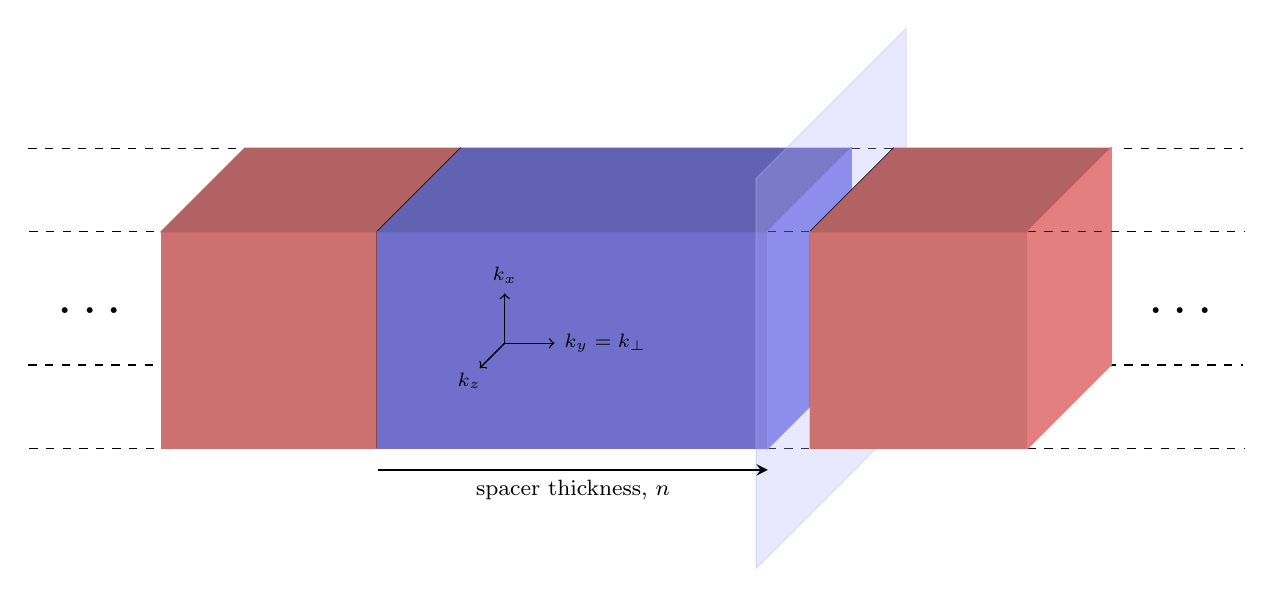
\begin{tikzpicture}[scale = 0.55,line width=0.5pt, scale = 5, node distance = 0.2]
\draw[dashed] (-1,0,0) -- (4.61,0,0);
\draw[dashed] (-1,1,0) -- (0,1,0);
\draw[dashed] (4.06,1,0) -- (4.61,1,0);
\draw[dashed] (2.8,1,0) -- (3,1,0);
\draw[dashed] (-0.61,0,1) -- (0,0,1);
\draw[dashed] (4,0,1) -- (5,0,1);
\draw[dashed] (2.8,0,1) -- (3,0,1);
\draw[dashed] (-0.61,1,1) -- (3,1,1);
\filldraw[red!45!white!80!black] (0,0,1) rectangle ++(1,1,0)node[scale=2, yshift=-0.5cm, color=black,xshift=-1.8cm]{\dots};
	\filldraw[red!45!white!70!black] (0,1,0) -- (1,1,0) -- (1,1,1) -- (0,1,1) -- cycle;
	\draw[line width=1pt] (1,0,1) -- (1,1,1) -- (1,1,0);
	\begin{scope}[xshift = 1cm]
	\filldraw[blue!45!white!80!black] (0,0,1) rectangle ++(1.8,1,0);
	\filldraw[blue!45!white!70!black] (0,1,0) -- (1.8,1,0) -- (1.8,1,1) -- (0,1,1) -- cycle;
	\filldraw[blue!45!white!90!black] (1.8,0,0) -- (1.8,1,0) -- (1.8,1,1) -- (1.8,0,1) -- cycle;
	\draw[dashed] (1.8,1,1)--(2,1,1);
	\filldraw[opacity = 0.3, blue!30] (1.9,-0.4,-0.4) -- (1.9,-0.4,1.4) -- (1.9,1.4,1.4) -- (1.9, 1.4,-0.4) --cycle;
\end{scope}
	\draw[line width=1pt] (3,0,1) -- (3,1,1) -- (3,1,0);
	\begin{scope}[xshift = 3cm]
		\filldraw[red!45!white!80!black] (0,0,1) rectangle ++(1,1,0)node[scale=2, yshift=-0.5cm, color=black, xshift=1cm]{\dots};
	\filldraw[red!45!white!70!black] (0,1,0) -- (1,1,0) -- (1,1,1) -- (0,1,1) -- cycle;
	\filldraw[red!45!white!90!black] (1,0,0) -- (1,1,0) -- (1,1,1) -- (1,0,1) -- cycle;
\end{scope}
\draw[dashed] (4,1,1) -- (5,1,1);
\draw[xshift = 1.2cm, yshift = 0.1cm,->] (0,0,0) -- (0,0,0.3) node[below left, xshift = 4pt, yshift = 2pt] {\scriptsize$k_z$};
\draw[xshift = 1.2cm, yshift = 0.1cm,->] (0,0,0) -- (0,0.23,0) node[above] {\scriptsize$k_x$};
\draw[xshift = 1.2cm, yshift = 0.1cm,->] (0,0,0) -- (0.23,0,0) node[right] {\scriptsize$k_y = k_\perp$};
\draw[thick, ->, > = stealth] (1,-0.1,1)--(2.8,-0.1,1) node[midway,below] { \footnotesize spacer thickness, $n$};

\end{tikzpicture}
\caption{\footnotesize Schematic of a \gls{cpp} trilayer. The red shaded areas are the semi-infinite leads, and the blue shaded area is the spacer. The spacer is grown from the LHS lead to thickness $n$, and for these calculations there is an imaginary cleavage plane passing between the $n$th spacer layer and the left surface of the RHS lead.}\label{fig:5th}
\end{figure}
\par The system comprises (see Figure \ref{fig:5th}) of a \gls{pm}, a metallic spacer and a \gls{sm} in its most minimal form. Often additional layers are required and in general the system is grown with \gls{cpp}. Thus it may be modelled that the magnetisation of the \gls{pm} lies in the $xz$ plane at an angle $\theta$ to the $z$ axis. The magnetisation of the \gls{sm} is held parallel to the $z$ axis. The closed-form \gls{sgf}'s of the leads may be calculated using Equation \eqref{SGF_AU}, the \gls{sgf} of the spacer and \gls{sm} are grown epitaxially using either Equation \eqref{adlayer} or Equation \eqref{bigG}. $\bf g_{\rm\scriptscriptstyle R}$ is the \gls{sgf} of the \gls{sm} in contact with the spacer, and $\bf g_{\rm\scriptscriptstyle L}$ is the \gls{sgf} of the outermost spacer layer.
The matrix of on-site potentials of the \gls{pm} have been rotated by $\theta$ as follows\textcolor{blue}{\textsuperscript{\cite{SC}}}
\begin{equation}
	\rm\bf u_{\rm 1 \theta}\; {\rm =}\; s^{\rm -1}u_{\rm 1 0}s
\end{equation}
where 
\begin{equation}
	{\bf s} = \begin{pmatrix} \cos(\frac{\theta}{2})&\sin(\frac{\theta}{2})\\-\sin(\frac{\theta}{2})&\cos(\frac{\theta}{2}) \end{pmatrix}
\end{equation}
It will be of interest to calculate the \gls{iec} of a system in the case of an applied bias. Unfortunately the integrand is not smooth with respect to energy, $\varepsilon$, so at least at this stage the zero-bias (equilibrium) case is considered.
At equilibrium, Equation \eqref{keldysh_1} yields the \gls{iec} by integrating with respect to $\theta$ from $0$ to $	\pi$
\begin{equation}\label{alt_exchange}
	{\rm J(n)}= \int_\theta d\theta \langle j_{n-1}\rangle_1 = \frac{1}{2\pi}\sum_{\bf k_\parallel}\int d\varepsilon \int_0^\pi d\theta\,\rm Re \, Tr \lbrace \bf (B-A)\bm\sigma\rbrace \mathnormal f(\varepsilon - \mu)
\end{equation}
The second method for describing \gls{iec} is derived directly from the thermodynamic potentials, which in equilibrium form is as follows
\begin{equation}\label{exchange}
	\rm J(n) = \frac{1}{n_\parallel}\sum_{\bf k_\parallel}Im\int_{-\infty}^{+\infty}{\mathnormal d}\varepsilon\;{\mathnormal f}(\varepsilon - \mu)F(\varepsilon, {\bf k_\parallel}, n)
\end{equation}
Where
\begin{equation}\label{F}
	\rm F = \frac{1}{\pi}\ln [det(\bf A_{\rm \scriptscriptstyle FM}^{\rm -1}A_{\rm \scriptscriptstyle AF})]
\end{equation}
Where $\bf A_{\rm \scriptscriptstyle FM}$ is in the \gls{fm} configuration $(\theta = 0)$, and $\bf A_{\rm \scriptscriptstyle AF}$ is in the \gls{af} configuration $(\theta = \pi)$\textcolor{blue}{\textsuperscript{\cite{rev3}}}. For computational efficiency purposes, these $2N\times2N$ matrices may be reduced to $N\times N$ matrices by separating $\bf A$ into it's spin up and spin down constituents $\bf A = \bm \alpha^\uparrow \bm\alpha^\downarrow$,
thus $\bm \alpha^\sigma = \bf(I - g_{\rm\scriptscriptstyle R}^\sigma t^\dag g_{\rm\scriptscriptstyle L}^\sigma t)^{\rm-1}$.
In this communication, efforts are directed at solving Equation \eqref{exchange}, which is again very numerically intensive if attempted to solve directly. Instead, two methods to solve Equation \eqref{exchange} are outlined here. The method of summing Matsubara frequencies is described initially\textcolor{blue}{\textsuperscript{\cite{mats}}}, followed by an outline of the \gls{spa}\textcolor{blue}{\textsuperscript{\cite{rev1}}}.
% A magnetic multilayer system is envisaged here comprising of a semi-infinite LHS magnetic lead with magnetisation in the $xz$ plane held parallel to the $z$ axis. One or more spacer materials grown to n atomic planes thick, the system is then completed with a semi-infinite RHS magnetic lead with magnetisation the $xz$ plane held at an angle $\theta$ from the z-axis. 
	\subsection{Method of Matsubara}
% The SGF of the leads are generated from Equation \eqref{SGF_AU}, the method of developing SGF's of the spacer layers varies depending on the method used to yield the exchange coupling in equilibrium (zero bias)
\par The Matsubara frequency method takes advantage of the fact that $\int_{-\infty}^{\infty}d\varepsilon$ can be integrated over the contour comprised of a semicircle who's diameter lies on the real line. This calculation is possible, since F($\varepsilon, \bf k_\parallel, \rm n)$ is analytic in this domain and $\longmapsto 0$, as $\varepsilon \longmapsto \pm \infty$\textcolor{blue}{\textsuperscript{\cite{tall}}}, and the Fermi function
has an infinite number of isolated singularities at $\varepsilon = \mu \pm (2m+1)kT\pi i$ for $m=0,1,2,\dots$, none of which lie on the real axis. $kT$ is the Boltzmann constant multiplied by temperature. The semicircle lies in the upper half plane, and so all singularities at $\gamma i$ for $\gamma < 0$ are discarded. 
The residues of $f(\varepsilon - \mu)$ lie at
	\begin{flalign}
	&\lim_{\omega \rightarrow(2m+1)\pi i}\frac{1}{1+e^{\omega}}=\\&\lim_{\omega \rightarrow(2m+1)\pi i}\frac{1}{\frac{1}{kT}e^{(\varepsilon-\mu)/kT}}=-kT
\end{flalign}
where $\omega = (\varepsilon-\mu)/kT$.
Thus
\begin{equation}\label{matsu}
	\int_{-\infty}^{+\infty}  d\varepsilon\; f(\varepsilon-\mu){\rm F}(\varepsilon, {\bf k}_\parallel, {\rm n})\equiv 2\pi i\left(-kT\sum_{m=0}^\infty {\rm F}\left(\mu{ + (2m+1) kT\pi i}, \rm\bf k_\parallel, \rm n\right)\right)
\end{equation}

	\tikzset{external/export next=false}
\begin{figure}[H]
	\centering
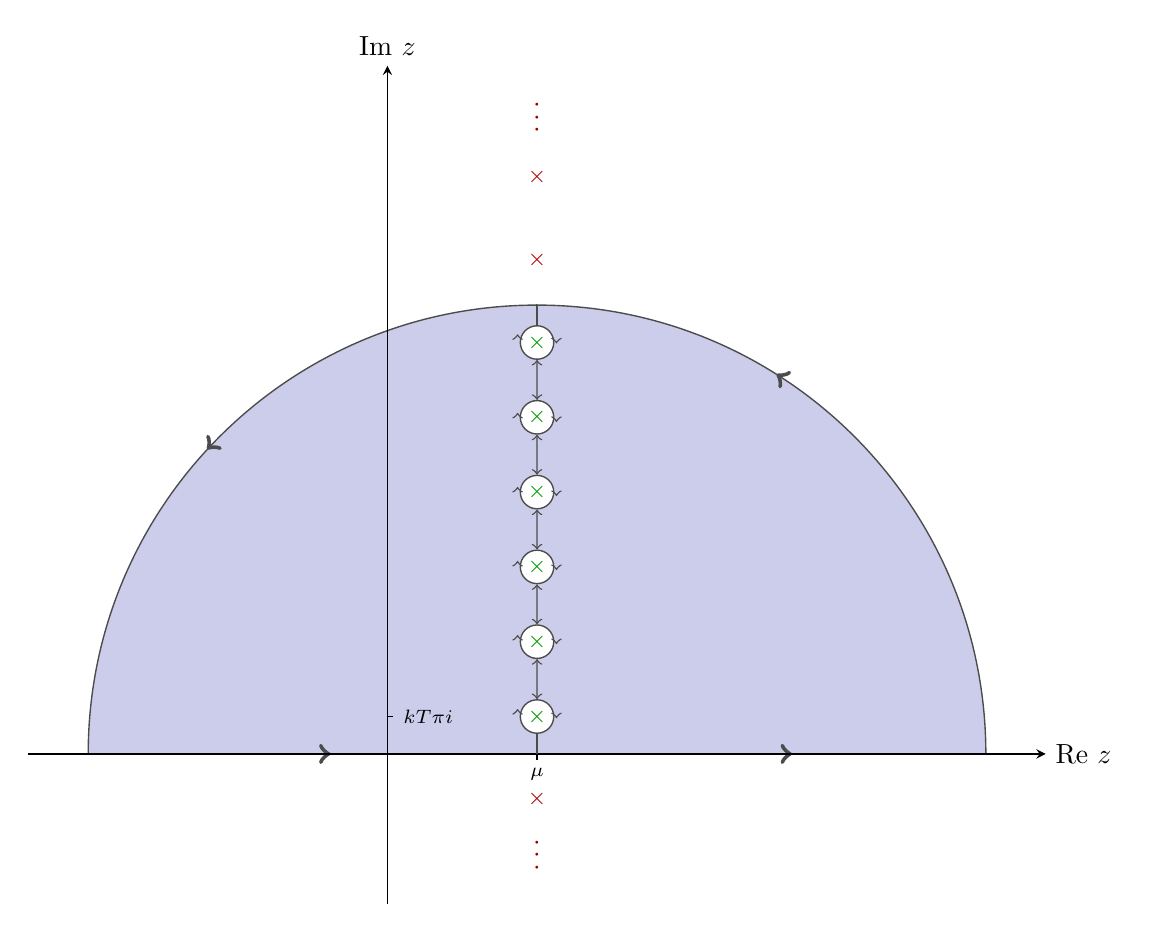
\begin{tikzpicture}[line width=0.5pt, scale = 3.8, node distance = 0.6]

	\filldraw[fill opacity = 0.2, color = blue!60!black, draw = black!70,
	decoration={markings,
		mark=at position 0.15 with{\arrow[ultra thick]{<}}, 
		mark=at position 0.42 with{\arrow[ultra thick]{<}}, 
		mark=at position 0.9 with{\arrow[ultra thick]{<}}, 
		mark=at position 0.7 with{\arrow[ultra thick]{<}}}, 
postaction = {decorate}] (-1,0) arc (180:0:1.5) -- cycle ;
	\draw[->,>=stealth] (-1.2,0) -- (2.2,0) node [right] {Re $z$};
	\draw[->,>=stealth] (0,-0.5) -> (0,2.3) node [above] {Im $z$};	
	\foreach \x in {0,1,...,5} 
		\draw
		[green!60!black,
			inner sep=1.2pt,
			% decoration={markings, 
			% mark=at position 0.5 with {\arrow{<}},
			% mark=at position 1.0 with {\arrow{<}}},
			% postaction={decorate}
		] 
		(0.5,{(.5+\x)/4}) node[circle,draw = black!70, fill = white](\x) {\footnotesize$\times$};

	\begin{scope}[draw = black!70, every node/.style={scale=.5}]
		% \pgfmathtruncatemacro{\yplusone}{\y + 1}
		\foreach \y in {0,1,...,4} 
		\pgfmathtruncatemacro{\yplusone}{\y + 1}
		\path[<->]   (\y)  edge   (\yplusone);
 \end{scope}

 \path[	 decoration={markings,
	 mark=at position 0.092 with{\arrow[black!70]{<}}, 
	 mark=at position 0.422 with{\arrow[black!70]{<}}, 
	 mark=at position 0.587 with{\arrow[black!70]{<}}, 
	 mark=at position 0.752 with{\arrow[black!70]{<}}, 
	 mark=at position 0.927 with{\arrow[black!70]{<}}, 
	 mark=at position 0.257 with{\arrow[black!70]{<}}}, 
	postaction = {decorate}
]
(0.565,0) -- (0.565,1.5);

 \path[	 decoration={markings,
	 mark=at position 0.1 with{\arrow[black!70]{>}}, 
	 mark=at position 0.43 with{\arrow[black!70]{>}}, 
	 mark=at position 0.595 with{\arrow[black!70]{>}}, 
	 mark=at position 0.76 with{\arrow[black!70]{>}}, 
	 mark=at position 0.935 with{\arrow[black!70]{>}}, 
	 mark=at position 0.265 with{\arrow[black!70]{>}}}, 
	postaction = {decorate}
]
(0.435,0) -- (0.435,1.5);

 \node (6) [red!70!black,above =of 5] {\footnotesize$\times$} ;
 \node (7) [red!70!black,above =of 6] {\footnotesize$\times$} ;
 \node (ellipsis) [red!60!black,above =of 7, yshift = -1pt, rotate=90, anchor=center] {\dots} ;
 \node (-1) [red!70!black,below =of 0] {\footnotesize$\times$} ;
 \node (ellipsisbelow) [red!60!black,below =of -1, yshift = 4pt, rotate=90, anchor=center] {\dots} ;
 \draw[black!70] (5) |- (0.5,1.5);
 \draw[black!70] (0) |- (0.5,0);
 \draw (0,0.125) -- (0.02,0.125) node[right]{$\scriptstyle{kT\pi i}$};
 \draw (0.5,0) -- (0.5,-0.02) node[yshift=-5pt]{\scriptsize$\mu$};
\end{tikzpicture}
\caption{\footnotesize
	Summation of Matsubara frequencies. The integral $\int_{-\infty}^{+\infty}$ is replaced with a semi-circular contour of infinite radius. Since $f(\varepsilon - \mu)$ has residue $-kT$ at each of its poles $\mu + (2m+1)kT\pi i$, for $m=0,1\dots$ , and $\rm F$ is analytic throughout the domain and converges for $\sum_{m=0}^\infty {\rm F}(\mu{ + (2m+1)kT\pi i}, \rm\bf k_\parallel, \rm n)$, the integral may be replaced by the summation 
	$2\pi i\Big(-kT\sum_{m=0}^\infty {\rm F}(\mu{ + (2m+1)kT\pi i}, \rm\bf k_\parallel, \rm n)\Big)$. The summation converges rapidly getting very good agreement at nine terms.
	}\label{fig:4th}
	
\end{figure}
The summation $\rm\bf k_\parallel$ in Equation \eqref{exchange} is over the two-dimensional Brillouin zone, which can be converted to an integral that can be evaluated numerically using quadrature routines detailed in the Appendix\textcolor{blue}{\textsuperscript{\cite{CP}}}, by making the following conversion
\begin{equation}\label{sum}
	\frac{1}{\rm n_\parallel}\sum_{\bf k_\parallel} \longrightarrow \frac{1}{\rm A_{\scriptscriptstyle BZ}} \int_{\bf k_\parallel}d^2 \bf k_\parallel
\end{equation}	
Where $\rm A_{\scriptscriptstyle BZ}$ is the area of the Brillouin zone.
Thus, the final form Equation \eqref{exchange} takes in this setting is
\begin{equation}
	{\rm{J(n)}}=-\frac{2\pi kT}{\rm A_{\scriptscriptstyle BZ}} \; {\rm Re}\sum_{m=0}^\infty\int_{\rm\bf k_\parallel} d^2 {\rm\bf k_\parallel}\big\{ {\rm F}\left(\mu{ + (2m+1)kT\pi i}, \rm\bf k_\parallel, \rm n\right)\big\}
\end{equation}
% The Green's function for the spacer layer are obtained by growing from the LHS lead using Equation \eqref{adlayer}. This is in order to maintain maximum numerical efficiency given that calculations of previous layers are stored in the process.
	\subsection{Stationary Phase Approximation}
	F($\varepsilon, \rm \bf k_\parallel, \rm n)$ is a quasi-periodic function of the continuous thickness n\site{rev3}. As such, F($\varepsilon, \rm \bf k_\parallel, \rm n)$ may be expanded in a Fourier-type series (exactly a Fourier series in the one-band model)
% The \acrfull{spa} method relies on the fact that 
\begin{equation}
	\rm F(\varepsilon, \bf k_\parallel, \rm n) = \sum_s \mathnormal{c_s(\varepsilon, {\bf k}_\parallel) e^{i\rm n \phi_s(\varepsilon, \bf k_\parallel)}}
\end{equation}
When this is substituted back into Equation \eqref{exchange}, it can be observed that for large n, the imaginary component of the integrand oscillates rapidly as a function of $\rm \bf k_\parallel$ and $\varepsilon$. As such, the only non-zero contributions to the $\rm \bf k_\parallel$ integral come from the neighbourhood of points in k-space where $\phi_s$ is stationary. Similarly, the only contributions to the $\varepsilon$ integral that don't cancel are those that arise near the sharp cut off that occurs at the chemical potential $\mu$.
\\[3mm]
The period of the \gls{iec} as a function of spacer thickness P $= \pi/\phi_s$ where $\phi_s = (a_1k_{\perp 1} + a_2k_{\perp 2} + \dots)$.
$c_s$ is complex, so may be expressed in polar form $c_s(\varepsilon, {\bf k_\parallel)} = |c_s(\varepsilon,{\bf k_\parallel)}|e^{i \psi_s (\varepsilon)}$ thus
\begin{equation}
	\rm F(\varepsilon, \bf k_\parallel, \rm n) = \sum_s \mathnormal{|c_s(\varepsilon, {\bf k_\parallel)}| e^{i\rm (n \phi_s(\varepsilon, {\bf k_\parallel})+ \psi_s(\varepsilon))}}
\end{equation}
$\phi_s$ is then expanded to second order in $\bf k_\parallel$ about the stationary point, ${\bf k}_\parallel^0$
\begin{multline}
	\phi_s({\bf k_\parallel}) = \phi_s({\bf k}_\parallel^0) + ({\bf k}_\parallel - {\bf k}_\parallel^0)^T\frac{\partial \phi_s}{\partial{\bf k}_\parallel }+ \frac{1}{2}({\bf k}_\parallel - {\bf k}_\parallel^0)^T(\partial^2\phi_s) ({\bf k}_\parallel - {\bf k}_\parallel^0) + \dots
\end{multline}
where $\partial \phi_s/\partial{\bf k}_\parallel,\,(\partial^2\phi_s)$ are $2\times2$ matrices, and $(\partial^2 \phi_s)$ is the Hessian matrix $(\partial^2\phi_s)_{x, z} \equiv \partial^2\phi_s/\partial{\rm \bf k_{\parallel \mathnormal x}}\partial{\rm \bf k_{\parallel \mathnormal z}}$. The essence of the \acrfull{spa} is to assume the contributions are largest when the phase is stationary. Thus ${\bf k}_\parallel^0$ is the solution to ${\partial \phi_s}/{\partial{\bf k}_\parallel } = 0$. Thus

\begin{multline}\label{stationary}
	{\rm J(n) = \frac{1}{\rm A_{\scriptscriptstyle BZ}}Im}\int_{-\infty}^{+\infty}d\varepsilon\;f(\varepsilon - \mu)\times \\ \sum_s{|c_s(\varepsilon,{\bf k}_\parallel^0)| e^{i{\rm (n} \phi_s(\varepsilon, {\bf k}_\parallel^0)+ \psi_s(\varepsilon))}}\int_{\bf k_\parallel}d^2 {\bf k}_\parallel \mathnormal e^{i(\frac{\rm n}{2}({\bf k}_\parallel - {\bf k}_\parallel^0)^T(\partial^2\phi_s) ({\bf k}_\parallel - {\bf k}_\parallel^0))}
\end{multline}
Where all terms not depending on $\bf k_\parallel$ have been commuted to the left of the integral in k-space, and where the following conversion has been used
\begin{equation}
	\frac{1}{\rm n_\parallel}\sum_{\bf k_\parallel} \longrightarrow \frac{1}{\rm A_{\scriptscriptstyle BZ}} \int_{\bf k_\parallel}d^2 \bf k_\parallel
\end{equation}	
Using a standard matrix result from Gaussian integration{\color{blue}{\textsuperscript{\cite{gauss}}}}, it can be shown that
\begin{equation}
	\int_{-\infty}^{+\infty} e^{(-\frac{1}{2}{\bf x^TAx})}d^n{\bf x}=\sqrt{\frac{(2\pi)^n}{{\rm det}A}}
\end{equation}
The RHS integral \eqref{stationary} can be converted into the form above
\begin{equation}\label{subs}
	\int_{-\infty}^{+\infty}d^2 {\bf k}_\parallel \mathnormal e^{i(\frac{\rm n}{2}({\bf k}_\parallel - {\bf k}_\parallel^0)^T(\partial^2\phi_s) ({\bf k}_\parallel - {\bf k}_\parallel^0))} \equiv\int_{-\infty}^{+\infty}d^2 {\bf y} \mathnormal e^{(-\frac{\rm 1}{2}{\bf y}^T( \frac{\rm n}{i}\partial^2\phi_s) {\bf y})}
\end{equation}
since scalars are commutative, and upon the substitution $({\bf k}_\parallel - {\bf k}_\parallel^0)={\bf y}$ with $d^2{\bf k}_\parallel = d^2({\bf y} + {\bf k}_\parallel^0)=d^2{\bf y}$.
Thus Equation \eqref{subs} yields
\begin{equation}
	\frac{2\pi}{\sqrt{-{\rm n}^2{\rm det}(\partial^2\phi_s)}} = \frac{2\pi\tau}{{\rm n}|{\rm det}(\partial^2\phi_s)|^{\frac{1}{2}}}
\end{equation}
Where $\tau = i$ if both eigenvalues of $(\partial^2\phi_s)$ are positive, $\tau = -i$ if both eigenvalues are negative and $\tau = 1$ when both eigenvalues differ in sign.
The \gls{iec} presently takes the form
\begin{equation}
	{\rm J(n)} = \frac{2\pi}{\rm nA_{\scriptscriptstyle BZ}}{\rm Im}\int_{-\infty}^{+\infty}d\varepsilon f(\varepsilon - \mu)\sum_{{\bf k}_{\parallel}^0}\sum_s\frac{\tau {|c_s(\varepsilon, {\bf k}_\parallel^0)| e^{i\left({\rm n} \phi_s(\varepsilon, {\bf k}_\parallel^0)+ \psi_s(\varepsilon)\right)}}}{\left|{\rm det}\left(\partial^2\phi_s(\varepsilon, {\bf k}_\parallel)\right)\right|^{\frac{1}{2}}}
\end{equation}
Next, $\psi_s$ and $\phi_s$ are expanded to first order about $\mu$
\begin{multline}
	\psi_s(\varepsilon) \approx \psi_s(\mu) + (\varepsilon - \mu)\psi_s'(\mu),\quad\quad \quad\quad \quad \phi_s(\varepsilon) \approx \phi_s(\mu) + (\varepsilon - \mu)\phi_s'(\mu)
\end{multline}
	Where all dashed terms are differentiated with respect to $\varepsilon$.
Making this substitution and bringing all terms that do not depend on $\varepsilon$ to the left of the integral yields
\begin{multline}
	{\rm J(n)} = \frac{2\pi}{\rm nA_{\scriptscriptstyle BZ}}\sum_{{\bf k}_{\parallel}^0}\sum_s {\rm Im}\left\{\tau e^{i\left({\rm n}\phi_s(\mu, {\bf k}_\parallel^0)+\psi_s(\mu)\right)} \times \rule{0cm}{0.8cm}\right.\\ \int_{-\infty}^{+\infty}d\varepsilon f(\varepsilon - \mu)\left. \frac{|c_s(\varepsilon, {\bf k}_\parallel^0)|e^{i\left( {\rm n} (\varepsilon - \mu)\phi_s'(\mu, {\bf k}_\parallel^0) + (\varepsilon - \mu)\psi_s'(\mu)\right)} }{\left|{\rm det}\left(\partial^2\phi_s(\varepsilon, {\bf k}_\parallel^0)\right)\right|^{\frac{1}{2}}}\right\}
\end{multline}
Next the substitution $x=(\varepsilon - \mu)/kT$ is made, thus $dx = d\varepsilon/kT$ and $f(\varepsilon - \mu)=\frac{1}{1+e^x}$
thus the integral takes the form
\begin{equation}
	kT\int_{-\infty}^{+\infty}dx \frac{|c_s(\varepsilon, {\bf k}_\parallel^0)|}{\left|{\rm det}\left(\partial^2\phi_s(\varepsilon, {\bf k}_\parallel^0)\right)\right|^\frac{1}{2}} \rule{0cm}{0.8cm} \frac{e^{ixkT\left({\rm n}\phi_s'(\mu, {\bf k}_\parallel^0)+\psi_s'(\mu)\right)}}{1+e^x}
\end{equation}
where upon inspection of the left hand term, given that it varies slowly with respect to $\varepsilon$ and lies entirely on the real line, $\varepsilon$ may be replaced by its first order term
\begin{equation}\label{dodgy}
	kT\frac{|c_s(\mu, {\bf k}_\parallel^0)|}{\left|{\rm det}\left(\partial^2\phi_s(\mu, {\bf k}_\parallel^0)\right)\right|^\frac{1}{2}}\rule{0cm}{0.8cm} \int_{-\infty}^{+\infty}dx \frac{e^{ixkT\left({\rm n}\phi_s'(\mu, {\bf k}_\parallel^0)+\psi_s'(\mu)\right)}}{1+e^x}
\end{equation}
using contour integration it can be shown that{\color{blue}{\textsuperscript{\cite{tall}}}}
\begin{equation}
	\int_{-\infty}^{+\infty} dx \frac{e^{ax}}{1+e^x} = \frac{\pi}{{\rm sin}(\pi a)}
\end{equation}
Thus Equation \eqref{dodgy} becomes
	\begin{multline}
			\frac{kT|c_s(\mu, {\bf k}_\parallel^0)|\pi}{\left|{\rm det}\left(\partial^2\phi_s(\mu,{\bf k}_\parallel^0)\right)\right|^\frac{1}{2} {\rm sin}\left(\pi i\left[{\rm n}\phi_s'(\mu, {\bf k}_\parallel^0)+\psi_s'(\mu)\right]kT\right)}\equiv\\\rule{0cm}{1cm} \frac{-ikT\pi|c_s(\mu, {\bf k}_\parallel^0)|}{\left|{\rm det}\left(\partial^2\phi_s(\mu,{\bf k}_\parallel^0)\right)\right|^\frac{1}{2} {\rm sinh}\left(\pi kT\left[{\rm n}\phi_s'(\mu, {\bf k}_\parallel^0)+\psi_s'(\mu)\right]\right)}
\end{multline}

\normalsize \justify \quad 
thus in full, the Stationary Phase Approximation of the \gls{iec} is

\begin{equation}
	{\rm J(n)} = -\frac{(2\pi)^2{kT}}{2{\rm nA_{\scriptscriptstyle BZ}}}\sum_s \sum_{{\bf k}_\parallel^0}{\rm Re}\left.\left(\frac{\tau  c_se^{i{\rm n}\phi_s}}{\vert {\rm det}(\partial^2\phi_s)\vert^\frac{1}{2}\sinh(\pi kT[n\phi_s '+\psi_s '])} \right) \right|_{\mu , {\bf k}_\parallel^0}\site{origspa}
\end{equation}
\subsubsection{1-band Simple Cubic model}
	Given that in this simple case the Fermi surface has a single sheet, the period P is equal to $\rm \pi/k_\perp$, and $\phi_s = 2s\rm k_\perp$\textcolor{blue}{\textsuperscript{\cite{rev3}}}.
	$\rm k_\perp$ is obtained by rearranging the dispersion relation
	\begin{equation}\label{dispersion}
		\rm \varepsilon = u + 2t\left(\cos(\bf k_\parallel \mathnormal a)+\cos(\rm k_\perp \mathnormal a)\right)	
	\end{equation}
	The summation over $\rm\bf k_\parallel$ is reduced to the sum of those values at which $\rm\bf k_\parallel$ is stationary. These values occur at $\rm d\phi_s/d\bf k_\parallel = \rm0$.
	Since
	\begin{equation}
		\rm k_\perp = \frac{1}{\mathnormal a}\cos^{-1}\Big(\frac{\varepsilon - u}{2t} - \cos(\bf k_\parallel \mathnormal a)\Big)
	\end{equation}
	Then
	\begin{equation}
		\rm \frac{\partial k_\perp}{\partial\bf k_\parallel} = -\frac{\sin(\bf k_\parallel\mathnormal a)}{\sqrt{-\left(\frac{\varepsilon - u}{2t}-\cos(\bf k_\parallel \mathnormal a)\right)^{\rm 2} -\rm 1}}
	\end{equation}
	Thus there is one stationary point, at $\rm\bf k_\parallel = 0$.
	The Fourier term
	\begin{equation}
		c_s= \frac{1}{\rm P} \int_{{\rm n}_0}^{{\rm n}_0+{\rm P}} d{\rm n \;F(n)}e^{- i\frac{2\pi s \rm n}{\rm P}}
	\end{equation}
	is integrated by utilising Equation \eqref{frac}, since this method is capable of handling non-integer n. The choice of $\rm n_0$ may be arbitrary.
	The Hessian matrix, $(\partial^2 \phi_s)$ is evaluated at the stationary point $\rm \bf k_\parallel^{\rm 0}$.
	$\tau=i$ when both eigenvalues of the Hessian matrix are positive, $\tau=-i$ when they are negative, and $\tau=1$ when they differ in sign.
	With these simplifications, the \gls{spa} may be restated as follows
\begin{equation}\label{SPA_2}
	{\rm J(n)} = -\frac{kT}{2{\rm n}}\sum_s \sum_{{\bf k}_\parallel^0}{\rm Re}\left.\left(\frac{\tau c_se^{2i{\rm n}sk_\perp}}{2s\vert \det(\partial^2k_\perp)\vert^{1/2}\sinh(\pi kT[2{\rm n}sk_\perp '+\psi_s '])} \right) \right\vert_{\mu , {\bf k}_\parallel^0}
\end{equation}
Where
\begin{equation}
	\rm k_\perp' = \left(\frac{\partial\varepsilon}{\partial k_\perp}\right)^{-1}=\left(-2t\mathnormal a\sin(k_\perp)\right)^{-1}
\end{equation}
and $\psi_s'$ is calculated numerically by comparing points on the gradient line over an infinitesimal distance such that the gradient is linear over these points.
The Hessian matrix evaluates in this case to
\\[3mm]
\begin{equation}
	(\partial^2\phi_s)_{x, z}=\begin{pmatrix} -\frac{a\cos(k_x a)}{\sqrt{-\cos^2(k_\perp a)+1}}+\frac{a\sin^2(k_x a)\cos(k_\perp a)}{(-\cos^2(k_\perp a)+1)^{1/2}}&\frac{a\sin(k_x a)\sin(k_z a)\cos(k_\perp a)}{(-\cos^2(k_\perp a))^{1/2}}\\\frac{a\sin(k_x a)\sin(k_z a)\cos(k_\perp a)}{(-\cos^2(k_\perp a))^{1/2}}&-\frac{a\cos(k_z a)}{\sqrt{-\cos^2(k_\perp a)+1}}+\frac{a\sin^2(k_z a)\cos(k_\perp a)}{(-\cos^2(k_\perp a)+1)^{1/2}} \end{pmatrix}
\end{equation}
\normalsize
\\[5mm]
Which is further simplified since $k_x, k_y = 0$. The results comparing the method of Matsubara, and \gls{spa} are presented in Figure \ref{fig:3rd}.
\\ [5mm]

	\tikzset{external/export next=false}
\pgfplotsset{width=5.6in}
\pgfplotsset{height=3in}
\begin{figure}[H]
	\centering
\begin{tikzpicture} 
	\begin{axis}[
			title=Interlayer Exchange Coupling,
			% title style = {xshift=-4ex},
			xlabel=$n$\quad \scriptsize{(atomic planes)},
			ylabel=$J(n)$ \, \scriptsize{(Ry)},
			scaled y ticks = false,
			ymin=-4e-5,
			ymax=6.5e-5,
			xmin=4,
			xmax=51,
		]
		\addplot[only marks, fill=red] table [col sep=comma] {mat_Mar.txt};\addlegendentry{Full numerical (Matsubara)}
		\addplot[green!80!black, line width=1pt] table [col sep=comma] {SPA_Mar.txt};\addlegendentry{Stationary Phase Approximation}
	\end{axis}

\end{tikzpicture}
\caption{\footnotesize
	Interlayer Exchange coupling given by both the Matsubara sum method, where the summation of Matsubara frequencies is taken as $\sum_0^9$, and \gls{spa}, where the summation of Fourier terms is taken over $\sum_{s=-5}^{s=5}$ though it can be observed that $c_0 = 0$. The potential in the leads $= -2.309Ry$ in the majority spin band and $=-0.95Ry$ in the minority band. The potential in the metallic spacer is $= -2.8Ry$. ${\rm t} = 0.5Ry$, $\mu= (0 + 1\times 10^{-5}i)Ry$ for \gls{spa}, and $(0+1\times 10^{-10}i)Ry$ for Matsubara. $kT = 1.9\times 10^{-3}Ry$ (room temperature).  Results calculated using C++11 with Clang compiler, utilising the Eigen library. Concurrency provided through OpenMP. }\label{fig:3rd}
	
\end{figure}
\subsection{Phase of Interlayer Exchange Coupling}
\par The Stationary phase approximation was analysed to ascertain phase dependence of \gls{iec}.
By applying perturbation and isolation techniques it became quickly apparent the phase was dominated by the first Fourier term (using direct complex Fourier series expansion agaist \gls{sgf}'s $\bf g$, this term is $c_{-1}$), in particular since this term is complex, it is the phase $\psi_s$ of the Fourier term that is of importance.
\par In order to understand the origin of this term more fully, it would be beneficial to negate the need to integrate over the spacer period, which is required using standard Fourier series expansion.
There are two alternative methods to obtain the Fourier components. The first involves taking an inverse \gls{fft}.
The second method replaces the \gls{sgf} with the \gls{mtgf} 
\begin{equation}\label{fn}
	\bm f_n = {\bf O}^{-1}\bullet {\bf g}_n
\end{equation}
Now recall $c_s$ are the Fourier components of F, Equation \eqref{F} with
\begin{equation}
	{\bf A}^{\alpha\beta} = ({\bf I - g}_{\scriptscriptstyle R}^{\alpha}{\bf t}^\dag {\bf g}_{\scriptscriptstyle L}^{\beta}{\bf t})^{-1}
\end{equation}
where $\alpha, \beta$ are the spin directions, so that
\begin{equation}
	{\rm F(n)} = F^{\uparrow\uparrow}({\rm n})+F^{\downarrow\downarrow}({\rm n}) - F^{\uparrow\downarrow}({\rm n})-F^{\downarrow\uparrow}({\rm n})
\end{equation}
with
\begin{equation}
	F^{\alpha\beta} = \ln\det({\bf A}^{\alpha\beta})^{-1}
\end{equation}
and it can be shown that\textsuperscript{\textcolor{blue}{\cite{com}}}
\begin{equation}\label{ftaylor}
	F^{\alpha\beta} \approx {\rm Tr}\left[\ln\left({\bf I}-\bm f_{\scriptscriptstyle R}^{\alpha}(0)\bm f_{\scriptscriptstyle L}^{\beta}({\rm n})\right)\right]
\end{equation}
where since $|\bm f| <1$, Equation \eqref{ftaylor} may be expanded as a Taylor series
\begin{equation}\label{fourierf}
	F^{\alpha\beta} \approx -{\rm Tr}\left[\bm f_{\scriptscriptstyle R}^{\alpha}(0) \bm f_{\scriptscriptstyle L}^{\beta}({\rm n})+\frac{1}{2}\left(\bm f_{\scriptscriptstyle R}^{\alpha}(0)\right)^2 \left(\bm f_{\scriptscriptstyle L}^{\beta}({\rm n})\right)^2+\frac{1}{3}\left(\bm f_{\scriptscriptstyle R}^{\alpha}(0)\right)^3 \left(\bm f_{\scriptscriptstyle L}^{\beta}({\rm n})\right)^3+\dots\right]
\end{equation}
but in the one band tight binding model, using Equations \eqref{glam}, \eqref{fn}, it is easy to see that $f_{\scriptscriptstyle L}^{\beta}({\rm n}) = f_{\scriptscriptstyle L}^{\beta}({\rm 0})e^{-2ik_\perp \rm n}$, since $\lambda_1 = e^{-ik_\perp}, \lambda_2 = e^{ik_\perp}$. Thus Equation \eqref{fourierf} can be re-expressed as follows
\begin{equation}\label{fs}
	F^{\alpha\beta} \approx -\sum_s \frac{1}{s}(f_{\scriptscriptstyle R}^\alpha f_{\scriptscriptstyle L}^\beta)e^{-2isk_\perp {\rm n}}
\end{equation}
where the independent variable is now dropped as the surface \gls{mtgf}'s are considered from here on.
\par Thus the \gls{mtgf}'s give a remarkably simple representation of the Fourier coefficients, $c_s$, giving a good platform to study the phase analytically.
\\[2mm] It is the first term that dominates the phase of \gls{iec}, $c_1$
\begin{equation}
	c_1^{\alpha\beta} = (f_{\scriptscriptstyle R}^\alpha f_{\scriptscriptstyle L}^\beta)
\end{equation}
Exploring an arbitrary \gls{mtgf} and using Equation \eqref{fn}
\begin{equation}
	f = -\frac{(\lambda_2{\rm t g} - 1)}{(\lambda_1 {\rm t g} - 1)}
\end{equation}
and utilising Equation \eqref{SGF_AU} together with knowledge that 
\begin{equation}
	{\bf O} = \begin{pmatrix} {\bf o}_1&{\bf o}_2\\{\bf \bm \tau o}_1\bm\Lambda_1&{\bf \bm \tau o}_2\bm\Lambda_2 \end{pmatrix}
\end{equation}
with ${\bf o}_1, {\bf o}_2$ denoting the upper-left and upper-right submatrices of $\bf O$, and $\bm \tau$ is the hopping matrix of the lead,
it is straightforward to show that 
$\rm g =\tau^{-1}\lambda_1$ with $\lambda_1$ being the eigenvalue of the lead.
This yields the following depending on whether the lead is an insulator or a conductor. In the case of a conductor
\begin{equation}\label{conductor}
	f = -\frac{(\frac{\rm t}{\tau}e^{i(k - \kappa)}-1)}{(\frac{\rm t}{\tau}e^{-i(k +\kappa)}-1)}
\end{equation}
and in the case of an insulator
\begin{equation}\label{insulator}
	f = -\frac{(\frac{\rm t}{\tau}e^{-\kappa} e^{ ik}-1)}{(\frac{\rm t}{\tau}e^{-\kappa} e^{-ik}-1)}
\end{equation}
Where the Greek characters refer to quantities of the leads, and the Roman characters refer to quantities of the spacer.
\par Complex analysis shows the system of most interest here is that of the insulator since the numerator is the complex conjugate of the denominator of $-f$, thus $|f|=1$, from which it follows that $|c_1| = 1$ establishing the dominance of this term. For the conducting spacer, $|f|<1$ since the sign of $\kappa$ always ensures the magnitude of the numerator is less than that of the denominator.
\par Similarly, with $\kappa$ being complex in the case of the conductor, the phase of the numerator of $-f$ will always be more advanced than that of the denominator. In the insulator the two phases are equal, and the total phase of the system is the sum of the phases of the denominator and numerator. It is thus expected the larger phase changes will be observed in an insulator, outlined in Fig. \ref{phase_drawing}.
\begin{figure}[H]
	\centering
	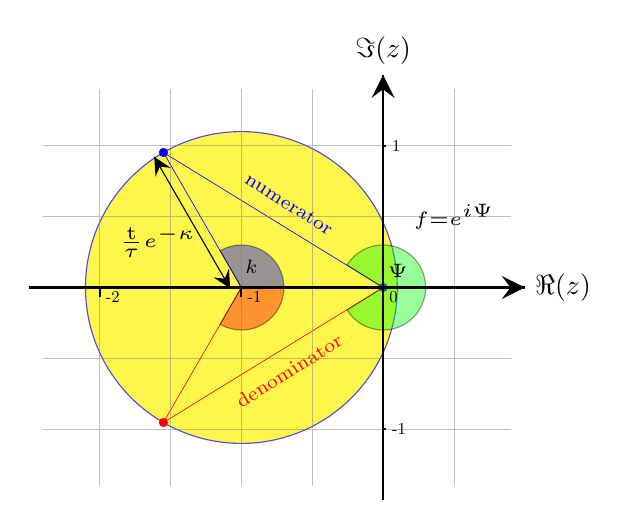
\begin{tikzpicture}[scale=1.8]
		\draw[blue,opacity = 0.7,fill=yellow] (-0.5,0) circle [radius=1.1cm];
		\draw[very thin,blue,fill=blue] (-0.5,0) -- +(120:1.1cm) circle[radius=0.03cm] -- node[midway, yshift=0.2cm, xshift = 0.2cm, rotate=-32]{\scriptsize numerator}(0.5,0) circle[radius = 0.03cm];
		\draw[very thin,red, fill=red] (-0.5,0) -- +(240:1.1cm) circle[radius=0.03cm] -- node[midway, yshift=-0.2cm,xshift = 0.2cm, rotate=32]{\scriptsize denominator} (0.5,0);
		\draw[black, fill = blue, opacity = 0.4] (-0.5,0) -- (-0.2,0) arc [start angle = 0, end angle = 120,radius = 0.3cm] node [black, opacity = 1, xshift = 0.4cm, yshift = -0.2cm] {$\scriptstyle k$}-- cycle;
		\draw[black, fill = red, opacity = 0.4] (-0.5,0) -- (-0.2,0) arc [start angle = 0, end angle = -120,radius = 0.3cm] -- cycle;
		\draw[black, fill = green, opacity = 0.4] (0.5, 0) -- node[opacity=1,black, scale=1.4, yshift=0.15cm, xshift=-0.06cm] {$\scriptscriptstyle\Psi$} (0.8, 0) arc [start angle = 0, end angle = 148, radius = 0.3cm] -- cycle;
		\draw[black, fill = green, opacity = 0.4] (0.5, 0) -- (0.8, 0) arc [start angle = 0, end angle = -148, radius = 0.3cm] -- cycle;
		\node[scale=1.4] at (1,0.5) {$\scriptscriptstyle f = e^{i\Psi}$};
		\draw[opacity = 0.5,step=.5cm,gray,very thin] (-1.9,-1.4) grid (1.4,1.4);
		\draw[decoration={markings,mark=at position 0 with
			{\arrow[xshift = 0.15cm,scale=2,>=stealth]{<}}, mark=at position 1 with {\arrow[scale=2, >=stealth]{>}}},postaction={decorate}] (-0.6, 0.03) -- +(120:1.03cm) node [scale=1.4, midway, yshift=-0.2cm,xshift=-0.3cm] {$\scriptscriptstyle\frac{\rm t}{\tau}e^{-\kappa}$};
		\draw [thick, decoration={markings,mark=at position 1 with
			{\arrow[scale=2,>=stealth]{>}}},postaction={decorate}](0.5,-1.5) -- (0.5, 1.5) node [above] {$\Im(z)$};
		\draw [thick, decoration={markings,mark=at position 1 with
			{\arrow[scale=2,>=stealth]{>}}},postaction={decorate}](-2,0) -- (1.5, 0) node [right] {$\Re(z)$};
		\foreach \x in {-2, -1, 0}
			\draw[thick] ({\x+0.5}, 0) -- ({\x+0.5}, -0.07) node [right, scale=0.6] {\x};
		\foreach \x in {-1, 1}
			\draw[thick] (0.5, \x) -- (0.52, \x) node[right, scale=0.6] {\x};
		\end{tikzpicture}
		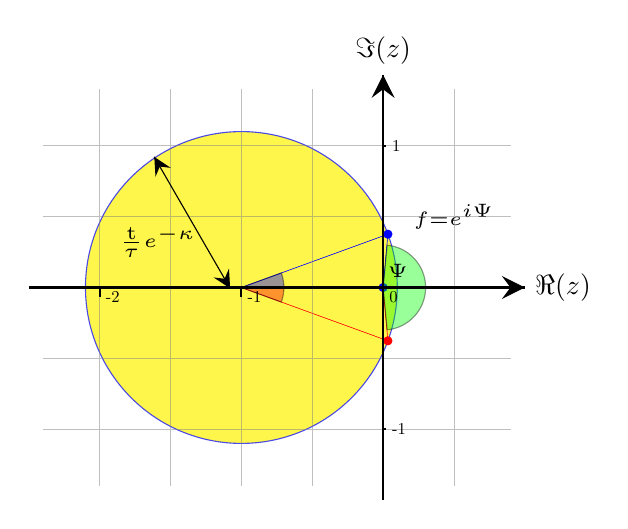
\begin{tikzpicture}[scale=1.8]
		\draw[blue,opacity = 0.7,fill=yellow] (-0.5,0) circle [radius=1.1cm];
		\draw[very thin,blue,fill=blue] (-0.5,0) -- +(20:1.1cm) circle[radius=0.03cm] -- (0.5,0) circle[radius = 0.03cm];
		\draw[very thin,red, fill=red] (-0.5,0) -- +(340:1.1cm) circle[radius=0.03cm] -- (0.5,0);
		\draw[black, fill = blue, opacity = 0.4] (-0.5,0) -- (-0.2,0) arc [start angle = 0, end angle = 20,radius = 0.3cm] -- cycle;
		\draw[black, fill = red, opacity = 0.4] (-0.5,0) -- (-0.2,0) arc [start angle = 0, end angle = -20,radius = 0.3cm] -- cycle;
		\draw[black, fill = green, opacity = 0.4] (0.5, 0) -- node[opacity=1,black, scale=1.4, yshift=0.15cm, xshift=-0.06cm] {$\scriptscriptstyle\Psi$} (0.8, 0) arc [start angle = 0, end angle = 84.5, radius = 0.3cm] -- cycle;
		\draw[black, fill = green, opacity = 0.4] (0.5, 0) -- (0.8, 0) arc [start angle = 0, end angle = -84.5, radius = 0.3cm] -- cycle;
		\node[scale=1.4] at (1,0.5) {$\scriptscriptstyle f = e^{i\Psi}$};
		\draw[opacity = 0.5,step=.5cm,gray,very thin] (-1.9,-1.4) grid (1.4,1.4);
		\draw[decoration={markings,mark=at position 0 with
			{\arrow[xshift = 0.15cm,scale=2,>=stealth]{<}}, mark=at position 1 with {\arrow[scale=2, >=stealth]{>}}},postaction={decorate}] (-0.6, 0.03) -- +(120:1.03cm) node [scale=1.4, midway, yshift=-0.2cm,xshift=-0.3cm] {$\scriptscriptstyle\frac{\rm t}{\tau}e^{-\kappa}$};
		\draw [thick, decoration={markings,mark=at position 1 with
			{\arrow[scale=2,>=stealth]{>}}},postaction={decorate}](0.5,-1.5) -- (0.5, 1.5) node [above] {$\Im(z)$};
		\draw [thick, decoration={markings,mark=at position 1 with
			{\arrow[scale=2,>=stealth]{>}}},postaction={decorate}](-2,0) -- (1.5, 0) node [right] {$\Re(z)$};
		\foreach \x in {-2, -1, 0}
			\draw[thick] ({\x+0.5}, 0) -- ({\x+0.5}, -0.07) node [right, scale=0.6] {\x};
		\foreach \x in {-1, 1}
			\draw[thick] (0.5, \x) -- (0.52, \x) node[right, scale=0.6] {\x};
	\end{tikzpicture}
	\caption{\footnotesize Depiction of Equation \eqref{insulator}, the \gls{mtgf} in the case of an insulating spacer. In each of the drawings, the blue point on the yellow disc indicates the numerator and the red point indicates the denominator. The blue shaded arc is the phase $k$, and the red shaded arc is the phase $-k$. The phase $\Psi$ is of interest here, depicted by the green shaded arc. It is apparent that should the radius $\frac{\rm t}{\tau}e^{-\kappa}$ become greater than $1$, as $k$ increases a large phase change will be observed. The drawing on the left which is fully labeled, shows the phase $\Psi$ is greater with more advanced $k$, than in the figure on the right with smaller $k$. It is evident in this scenario that a $2\pi$ phase change may be observed, as $k$ passes from $0$ to $\pi$. Alternatively, a large phase change of $\Psi$ can also be observed as the radius of the yellow disc, $\frac{\rm t}{\tau}e^{-\kappa}=r$ moves from $r<1$ to $r\ge1$, when $k$ is small.}\label{phase_drawing}
\end{figure}
\par With this theory in account, a one dimensional, \gls{sc} one band model was used to compute the \gls{iec} at different ratios of hopping in the leads compared to the spacer. The results are shown in Fig. \ref{phase_graph}. The system explored has a weak insulating spacer so that the oscillations of the \gls{iec} were only slightly damped. Fig. \ref{phase_graph} shows a strong phase dependence on the hopping ratios.
\pgfplotsset{height=4in}

	\begin{figure}[H]
\begin{tikzpicture} 
	\begin{axis}[
			title= Exchange Coupling,
			xlabel=$n$\quad \scriptsize{(atomic planes)},
			ylabel=$J(n)$ \, \scriptsize{(Ry)},
			xmin=10,
			xmax=50,
			scaled y ticks = false,
			legend entries = {$SPA \quad t_{lead} = 0.15$,$Full \quad t_{lead} = 0.15$, $SPA \quad t_{lead} = 0.25$, $Full \quad t_{lead} = 0.25$},
		]
		\addplot[blue] table [col sep=comma] {SPA_15_1D.txt};
		\addplot[purple] table [col sep=comma] {Mat_15_1D.txt};
		\addplot[red] table [col sep=comma] {SPA_25_1D.txt};
		\addplot[green] table [col sep=comma] {Mat25_1D.txt};
	\end{axis}
\end{tikzpicture}
\caption{\footnotesize This figure shows the \gls{iec} in the one dimensional case, as a function of spacer thickness for two different hoppings in the leads in Rydbergs, showing the full numerical results and \gls{spa} calculations.
The potential in the leads $= -0.7Ry$ in the majority spin band and $=-0.5Ry$ in the minority band. The potential in the spacer is $= -0.79Ry$, the hopping in the spacer is ${\rm t} = 0.4Ry$, $\mu= (0 + 1\times 10^{-5}i)Ry$ for \gls{spa}, and $(0+1\times 10^{-10}i)Ry$ for Matsubara. $kT = 1.9\times 10^{-3}Ry$ (room temperature).  Results calculated using C++11 with Clang compiler, utilising the Eigen library. Concurrency provided through OpenMP.
}\label{phase_graph}
\end{figure}
With the potentials used in Fig. \ref{phase_graph}, firstly considering the case when the hopping in the leads is $0.15Ry$, the leads behave as insulators in the majority spin band and $f^\uparrow$ has the radial term (introduced in Fig. \ref{phase_drawing}) $r\approx 0.60$. In the minority spin band, the leads also behave as insulators with $f^\downarrow$ having radial term $r\approx 0.89$. 
\par Now considering the case when the hopping in the leads is $0.25Ry$, the leads behave as insulators in the majority spin band and $f^\uparrow$ has radial term $r\approx 0.67$. In the minority spin band, the leads have in the strictest sense become conducting, but this case is in fact the boundary term where Equations \eqref{conductor}, \eqref{insulator} are equal. Here $f^\downarrow$ has radial term $r=1.60$.
\par It is since in the minority spin band the radial term in $f$ changes from $r\approx0.89$ to $r=1.60$, that the phase change in Fig. \ref{phase_graph} is observed.

	\section{Conclusion \& Future Developments}
	\par This communication has outlined the method of tight-binding and the Green's function formalism and applied these to describe the \gls{iec}. The \gls{iec} was given in its general form, then an analytical form was derived. Analysis of the analytic form (\gls{spa}) led to qualitative descriptions of the governance of phase in \gls{iec}. 
	\\\par The discovery by Umerski\textsuperscript{\textcolor{blue}{\cite{AUphase}}} regarding the $2\pi$ topologically protected phase shift has opened up an exciting area of research, with potential application to low energy \gls{mram} devices. This is an end-goal that has been under active research for some time, though effort has been directed to \gls{stt}-\gls{mram} , which at this stage requires a large current density to enable switching. \gls{mram} by virtue of its design, is non-volatile which is also of practical significance.
	\\\par Future developments will include comprehending and making use of realistic tight-binding models with as many as nine bands, to make fully realistic calculations of systems to explore the phase dependence of the \gls{iec}.
In order to simulate 'realness', surface roughness will be modeled and a thin switching layer will be considered.
Different realistic structures will be modeled to explore the suitability of certain materials, though due to limitations of theory, these will of course be crystalline.
\\\par Due to the required gate voltage, the Matsubara frequency method will no longer be valid as a means of calculating \gls{iec}.
Thus a full numerical computation requires direct integration over energy and two-dimensional $k$-space. This is very numerically intensive and the integrand as a function of energy is not smooth.
To make this problem more tractable, the Author has been developing a quadrature routine that is doubly adaptive and takes advantage of Brillouin zone symmetries.
More details are given in the Appendix.

	\appendix
	\section{Numerical Integration}
	\subsection{Cunningham's Special Points set}\label{points}
	In his 1974 paper\textcolor{blue}{\textsuperscript{\cite{CP}}}, Cunningham describes the special points set that minimises the required function calls for converged integration of the \gls{2dbz}, for a number geometries. His work follows that of Chadi and Cohen\textcolor{blue}{\textsuperscript{\cite{CC}}}, where the integrable function is expanded as a Fourier series
	\begin{equation}\label{cp}
		f({\bf k})=f_0 +\sum_{m=1}^\infty f_m A_m({\bf k})
	\end{equation}
	with
	\begin{equation}
		A_m({\bf k})=\sum_{|{\bf R}|=c_m}e^{i\bf k \cdot R},\qquad m=1,2,\dots
	\end{equation}
	The exact average over the \gls{2dbz} is equal to $f_0$, since the second term in Eq. \eqref{cp} vanishes. As such, upon imposing the restrictions
	\begin{equation}\label{A}
		\sum_i \alpha_i A_m({\bf k})=0, \qquad m = 1,2,\dots,N 
	\end{equation}
	\begin{equation}
	\sum_i \alpha = 1	
	\end{equation}
	Where N is the number of functions $A_m({\bf k})$ that satisfy Eq. \eqref{A}.\\
	They found the most efficient means of integrating over the \gls{2dbz} was by
	\begin{equation}
		f_0 = \sum_i \alpha_i f({\bf k}_i) - \sum_{m> N}^\infty f_m \sum_i \alpha_i A_m({\bf k}_i)
	\end{equation}
	Though in primitive-rectangular or square lattices, a set of generating wave vectors could always be found that zeros all functions $A_m({\bf k})$, so the algorithm reduces to a 'mesh' of equally spaced points, displaced from the origin by $a(\frac{1}{2},\frac{1}{2})$ where $a$ is the distance between the neighbouring points.
	\\[2mm] For these simple lattice types, the integral is performed as follows;
	\begin{equation}
		\iint_{\rm BZ}f({\rm k}_x, {\rm k}_z) d{\rm k}_xd{\rm k}_z= F_N
	\end{equation}
	where in the case of the square lattice
	\begin{equation}\label{CPsquare}
		F_N =\frac{8A_{\rm BZ}}{N^2}\sum_{n=0}^{2N}\left(\sum_{m=0}^{n-1} f\left(\frac{n\pi}{2Na}, \frac{m\pi}{2Na}\right)\delta_{p 1}\delta_{r 1}+\frac{1}{2}f\left(\frac{n\pi}{2Na}, \frac{n\pi}{2Na}\right)\delta_{p 1}\delta_{r 1}\right)
	\end{equation}
	and in the case of the primitive rectangular lattice
	\begin{equation}\label{CPrectangle}
		F_N =\frac{4A_{\rm BZ}}{N^2}\sum_{n=0}^{2N}\sum_{m=0}^{2N} f\left(\frac{n\pi}{2Na}, \frac{m\pi}{2Nb}\right)\delta_{p 1}\delta_{r 1}
	\end{equation}
	where $p \equiv n\pmod 2$ and $r \equiv m\pmod 2$. $\delta_{x y}$ is the Kronecker Delta where $\delta_{x y} = 1$ if $x=y$ and $\delta_{x y} = 0$ if $x\neq y$.
	\\\par Here $N$ is the number of points used along the $k_x\,(k_z)$ axis. In the irreducible segment of the square lattice, this is the largest number of points along that axis. In a primitive-rectangular lattice, no such distinction exists. $a,\,b$ are lattice constants with $a=b$ in the case of the square lattice.

	\subsection{Author's 2D Brillouin Zone integration method}
	\qquad The method outlined in Subsection \ref{points} is the most efficient algorithm for integrating over the \gls{2dbz} by minimising the number of regularly spaced points required. The form given by Cunningham requires the user to determine whether convergence has been achieved, repeating with more points if necessary. If the function is slow to converge, this can be quite time consuming. 
	The Author has made two developments to the results of Subsection \ref{points}. In both cases 'automatic' techniques are used, where if convergence hasn't been met, new points are used without discarding the work already done. In each case, the algorithm is for the square lattice, though it is easily extendible (and easier to write) to the primitive rectangular lattice. 
	\\[2mm]
	The simplest of these two techniques is as follows: 
	\\[2mm]where in the case of the square lattice
\begin{multline}\label{auto_square}
		F_{3^qN} =\frac{8A_{\rm BZ}}{(3^\alpha N)^2}\sum_{q=0}^\alpha\sum_{n=0}^{2(3^q)N}\left(\sum_{m=0}^{n-1} f\left(\frac{n\pi}{2(3)^qNa}, \frac{m\pi}{2(3)^qNa}\right)\delta_{p 1}\delta_{r 1}l\right.\\\left.+\frac{1}{2}f\left(\frac{n\pi}{2(3)^qNa}, \frac{n\pi}{2(3)^qNa}\right)\delta_{p 1}\delta_{r 1}l\right)
	\end{multline}
	and in the case of the primitive-rectangular lattice

	\begin{equation}\label{auto_rect}
		F_{3^qN} =\frac{4A_{\rm BZ}}{(3^\alpha N)^2}\sum_{q=0}^\alpha\sum_{n=0}^{2(3^q)N}\sum_{m=0}^{2(3^q)N} f\left(\frac{n\pi}{2(3)^qNa}, \frac{m\pi}{2(3)^qNb}\right)\delta_{p 1}\delta_{r 1}l
	\end{equation}

	Where $q=\alpha$ is an integer such that $\abs{1-\abs{\frac{F_{2^{\alpha-1} N}}{F_{2^\alpha N}}}} \leq \delta$ and $\delta$ is the required relative error. $l=1$ if $ {n\pmod 3}=0 \land {m\pmod 3}=0$ and $l=0$ otherwise.
	These equations are essentially revisions to equations \eqref{CPsquare} \& \eqref{CPrectangle}. It can be observed that the combination of $l$ and the summation over $q$ means that points are 'recycled' rather than recalculated, hence optimising efficiency. $N$ is the number of points used in each meridian at the start of the algorithm with different starting values leading to different completion times. Though per function, the optimal value $N$ is only obtained by trial and error, it is recommended that the user starts with small $N$. The difference in completion time depending on $N$ is not negligible; if $\phi$ is the time it takes to complete with $\alpha=c$ for some integer $c$, then $9\phi$ is the total completion time when $\alpha = c+1$.
	\\\par A case can be argued whether the efficiency of reusing the previously calculated points is favourable to simply quadrupling (in for example the primitive rectangle) the number of points. By reusing the previous points, the next pass uses nine times as many points, as indicated above. Upon quadrupling the number of points and discarding the previous work, there is a possibility convergence may be achieved more quickly, however this method penalises performance for allowing automatic convergence. Following the analysis of W. H. Press \textit{et. al.}\textsuperscript{\textcolor{blue}{\cite{numrec}}} and adapting to the square lattice indicates on average, the unnecessary work required for Equation \eqref{auto_square} versus that of the quadrupling routine is a scaling of $\sqrt{\frac{15}{7}} \approx 1.46$ whereas the penalty incurred for not reusing the points in the quadrupling routine is variable, depending on the number of iterations and starting number of points, ranging from a performance factor of $1.66$ to $1.33$. The factor of $1.33$ arises from a high number of starting points used, and one further pass being required. The factor of $1.66$ arises from a low starting number of one point and a low number of passes required. For a low starting number and a high number of passes required, the factor converged to $1.5$. Therefore the median ratio of $1.46:1.5$ puts Equation \eqref{auto_square} as more favourable. This is qualitatively useful, as it further emphasises the usefulness of being able to start with a small number of points, whereas in the alternative scheme, the penalty is compounded if multiple passes are required.
	\\\par Applying the above analysis to the primitive rectangle, the unnecessary work required for Equation \eqref{auto_rect} versus that of the quadrupling routine is a scaling of $1.5$ whereas the penalty incurred in the quadrupling method for not reusing points is a scaling of $1.33$ on the number of evaluations required, if only one further pass is performed (no matter what the starting number of points is, in contrast with the square lattice). For a large number of passes, the total performance penalty converges to $1.5$ thus in this case the total work required is on average equivalent. In this case, it is worth using the quadrupling technique if the integral is expected to converge quickly, and Equation \eqref{auto_rect} otherwise.
\pgfplotsset{width=3in}
\pgfplotsset{height=3in}
	\tikzset{external/export next=false}
\begin{figure}[H]
\begin{tikzpicture} 
	\begin{axis}[
			title=First pass,
			% title style = {xshift=-4ex},
			ylabel=$k_z$,
			ylabel style={rotate=-90},
			xlabel=$k_x$,
			xtick={0,1.5708,3.14159},
			xticklabels={$0$,$\frac{\pi}{2}$,$\pi$},
			ytick={0,1.5708,3.14159},
			yticklabels={$0$,$\frac{\pi}{2}$,$\pi$},
			ymin=-0.2,
			ymax=3.34,
			xmin=-0.2,
			xmax=3.34,
		]
		\addplot[only marks, fill=red] table [col sep=comma] {phase1.txt};
	\end{axis}
	\hspace{3.2in}
	\begin{axis}[
			title=Second pass,
			% title style = {xshift=-4ex},
			ylabel=$k_z$,
			ylabel style={rotate=-90},
			xlabel=$k_x$,
			xtick={0,1.5708,3.14159},
			xticklabels={$0$,$\frac{\pi}{2}$,$\pi$},
			ytick={0,1.5708,3.14159},
			yticklabels={$0$,$\frac{\pi}{2}$,$\pi$},
			ymin=-0.2,
			ymax=3.34,
			xmin=-0.2,
			xmax=3.34,
		]
		\addplot[only marks, fill=blue] table [col sep=comma] {phase2.txt};
	\end{axis}

\end{tikzpicture}
\caption{\footnotesize
Author's 'automatic' CSP routine with $N = 3$ and $a=1$ showing the first pass on the left ($q=0$) and the second pass on the right ($q=1$). The figure illustrates how there is no penalty incurred when the number of points is increased, where the total number of points is the sum of both frames. Each point along the diagonal has half the weighting of the remaining points.}
\end{figure}
The coded routine requires the following input parameters;
\\
\storestyleof{itemize}
\begin{listliketab}
	\begin{tabular}{lll}
	\textbullet &The starting number of points per meridian, $N$ &{\it must be an integer}\\
	\textbullet &The relative error tolerance, $\delta$ &{\it in decimal form}\\
	\textbullet &The maximum number of points per meridian &{\it must be an integer}\\
	\textbullet &The lattice constant, $a$ & \\
	\textbullet &Any number of further parameters to be forwarded to $f$&\\
	\end{tabular}
\end{listliketab}
\par
The second more sophisticated technique is presently under development. It is a doubly adaptive routine which splits the integrand with regard to both dependent variables testing for convergence on each side. Any converged sides remain without further calculations, and any unconverged sides are split further until convergence is achieved. The routine is iterative, creating a starting number of points then checking for convergence along $k_x$ then along $k_z$ where any splitting along $k_z$ invokes checks along the new points in $k_x$ created. The algorithm requires second order recursive functions.
The routine requires the following input parameters;

\storestyleof{itemize}
\begin{listliketab}
	\begin{tabular}{lll}
	\textbullet &The recursion depth cap &{\it must be an integer}\\
	\textbullet &The relative error tolerance &{\it in decimal form}\\
	\textbullet &The starting number of points per meridian &{\it must be an integer}\\
	\textbullet &The lattice constant, $a$ & \\
	\textbullet &Any number of further parameters to be forwarded to $f$&\\
	\end{tabular}
\end{listliketab}

In each case, the routine has been concisely written as a header file within C++14 made callable for a number of different types including the Tux Family Eigen container type. The compiler is able to infer the type required in the routine from the return type of the function forwarded in the parameter list within the initial calling sequence. The routine makes use of perfect forwarding of r-value references to improve efficiency.
Forwarding of an arbitrary number of parameters to $f$ is made possible by means of variadic templates.

% Table 1 shows benchmarking timings from the authors machine\footnote{Intel Core i3-3120M CPU @ 2.50GHz, 4GB RAM} between the new adaptive method, and the standard CSP method. The results in each case are converged with relative error $\delta \leq 3\%$. 
% The full routine is not displayed here, as it is very technically dense and requires knowledge of C++ and various techniques therein. It is however, available on request. create true CP routine to benchmark
% \\[8mm]
% \footnotesize
% \begin{center}
% \begin{tabular}{cccc}\toprule
% 	Computation& \parbox{3cm}{\centering Return type of integrand}& \parbox{3cm}{\centering Time to output results using standard CP}& \parbox{3cm}{\centering Time to output results using adaptive CP}\\
% \midrule
% \parbox{3cm}{\centering Local density of states of a semi-infinite crystal}& Real (double)& 28 seconds& 3 seconds\\[8mm]
% \parbox{3cm}{\centering Exchange Coupling using summation of Matsubara Frequencies}& \parbox{3cm}{\centering Container of type complex double}& 79 seconds& 3 seconds\\[8mm]
% \parbox{3cm}{\centering Keldysh formalism (slow to converge)}& \parbox{3cm}{\centering Container of type real (double)}& 4 minutes& 3 minutes\\
% \bottomrule
% \end{tabular}
% \end{center}

\normalsize
\begingroup
\let\clearpage\relax
\bibliography{exchange.bib}
\bibliographystyle{ieeetr}
\endgroup
\end{document}
